\documentclass[10pt,twocolumn]{article}
\usepackage[margin=0.75in]{geometry}
\usepackage{graphicx}
\usepackage{booktabs}
\usepackage{hyperref}
\usepackage{amsmath}
\usepackage{caption}
\usepackage{float}
\usepackage{balance}

% Allow LaTeX to place more floats per page and reduce gaps
\renewcommand{\topfraction}{0.9}
\renewcommand{\bottomfraction}{0.9}
\renewcommand{\textfraction}{0.08}
\renewcommand{\floatpagefraction}{0.8}
\setcounter{topnumber}{4}
\setcounter{bottomnumber}{4}
\setcounter{totalnumber}{8}
\setlength{\intextsep}{6pt plus 2pt minus 2pt}
\setlength{\floatsep}{8pt plus 2pt minus 2pt}
\setlength{\textfloatsep}{10pt plus 2pt minus 2pt}

\title{Gateway Complications: Mining Comorbidity Networks to Reveal\\Complication Clusters and Demographic Disparities in Type~2 Diabetes}

\author{
Marvin Osei-Kuffour (\texttt{moseikuffour@usf.edu}) \and Javier Varela (\texttt{javiervarela@usf.edu})\\
CIS 4930 / CAI 5155 --- Network Analysis \& ML with Graphs\\
University of South Florida\\
}

\date{Fall 2026}

\begin{document}
\maketitle

% ======================================================================
% SECTION 1: INTRODUCTION
% ======================================================================
\section{Introduction}

Type~2 diabetes mellitus (T2D) affects over 37 million Americans and rarely occurs in isolation~\cite{barabasi2011}.
Patients with T2D accumulate a constellation of comorbidities---hypertension, chronic kidney disease, cardiovascular conditions---that interact in ways that are difficult to capture with traditional epidemiological methods.
Understanding which conditions cluster together, which diagnoses act as bridges between otherwise separate disease domains, and whether these patterns differ across demographic groups is essential for improving clinical decision-making and resource allocation.

Network analysis provides a principled framework for studying these relationships.
By representing conditions as nodes and their co-occurrence within patients as weighted edges, we can apply social network analysis (SNA) techniques to reveal hidden structure in electronic health record (EHR) data.

In this project, we construct and analyze comorbidity networks for T2D patients extracted from the EHRShot dataset~\cite{wornow2023}.
Specifically, we address three research questions:

\begin{enumerate}
    \item \textbf{What comorbidity communities exist among T2D patients, and what clinical domains do they represent?}
    \item \textbf{Which diagnoses act as bridges between otherwise separate comorbidity clusters, serving as potential early markers of disease progression?}
    \item \textbf{How do comorbidity network structures differ across demographic subgroups (age, sex)?}
\end{enumerate}

Our analysis reveals 12 comorbidity communities organized around clinically coherent disease domains, identifies 52 bridge diagnoses connecting these communities, and demonstrates measurable structural differences across age and sex subgroups.
These findings provide a data-driven map of the T2D complication landscape that could inform comorbidity screening priorities.


% ======================================================================
% SECTION 2: RELATED WORKS
% ======================================================================
\section{Related Works}

\textbf{Hidalgo et al.\ (2009)}~\cite{hidalgo2009} introduced the phenotypic disease network (PDN), constructing a network where nodes are diseases and edges represent statistically significant co-occurrence in the same patients.
They used Relative Risk as edge weight and demonstrated that connected diseases share genetic origins.
Our work follows their co-occurrence methodology but focuses specifically on T2D patients and uses Jaccard similarity for normalization, which is bounded $[0,1]$ and more stable for varying prevalence levels.

\textbf{Jensen et al.\ (2014)}~\cite{jensen2014} built temporal disease trajectories from 6.2 million Danish patients, using directed edges based on first-occurrence ordering to identify statistically significant disease progressions.
We adapt their first-occurrence temporal methodology to construct a directed transition network within our T2D cohort, enabling identification of gateway conditions that precede downstream complications.

\textbf{Barab\'asi et al.\ (2011)}~\cite{barabasi2011} established the theoretical framework of network medicine, arguing that diseases should be studied through their molecular and phenotypic network relationships rather than in isolation.
Our project operationalizes this framework by applying community detection and centrality analysis to a disease co-occurrence network, treating the comorbidity landscape as an interconnected system.

\textbf{Blondel et al.\ (2008)}~\cite{blondel2008} proposed the Louvain algorithm for community detection, which optimizes modularity through iterative merging of nodes into communities.
We apply Louvain to partition our comorbidity network into clinically interpretable clusters, enabling identification of disease domains and the bridge diagnoses that connect them.

\textbf{Guimer\`a \& Amaral (2005)}~\cite{guimera2005} introduced the participation coefficient to classify nodes by their role in modular networks.
Nodes with high participation coefficients distribute their connections across multiple communities, functioning as connectors.
We combine participation coefficient with betweenness centrality to identify bridge diagnoses---conditions that link separate comorbidity clusters.

\textbf{Wornow et al.\ (2023)}~\cite{wornow2023} released EHRShot, a benchmark of de-identified longitudinal EHR data from Stanford Medicine in the OMOP Common Data Model format.
EHRShot provides the standardized vocabulary and concept hierarchies that enable our cohort definition and network construction.

Our work differs from prior studies by (1) focusing specifically on T2D comorbidity structure rather than population-wide disease networks, (2) combining community detection with bridge diagnosis identification and demographic stratification in a single analysis, and (3) using the OMOP-standardized EHRShot dataset with concept hierarchy expansion for rigorous cohort definition.


% ======================================================================
% SECTION 3: NETWORK CONSTRUCTION DETAILS
% ======================================================================
\section{Network Construction Details}

\subsection{Dataset and Cohort Selection}

We use the EHRShot dataset~\cite{wornow2023}, which contains longitudinal EHR data in the OMOP Common Data Model format.
Our analysis uses three core tables: \texttt{condition\_occurrence} (1,790,586 records), \texttt{person} (6,739 patients), and \texttt{concept\_ancestor} (vocabulary hierarchy).

We define the T2D cohort using SNOMED concept ID 201826 (``Type 2 diabetes mellitus'') and expand to all 18 descendant concepts via \texttt{concept\_ancestor}, following standard OHDSI cohort definition methodology~\cite{barabasi2011}.
A patient enters the cohort if they have $\geq 1$ condition record matching any T2D descendant concept.
This yields \textbf{1,354 patients} (22\% of EHRShot patients with condition records).

\subsection{Preprocessing}

For each cohort patient, we extract \textit{all} condition records (not only diabetes-related ones), since our research question concerns the full comorbidity landscape.
We apply three filters:

\begin{enumerate}
    \item \textbf{Standard concepts only:} Keep conditions where \texttt{standard\_concept = `S'} and \texttt{domain\_id = `Condition'}, avoiding double-counting from unmapped source codes.
    \item \textbf{Deduplication:} Remove duplicate records where the same patient has the same condition on the same date (administrative duplicates).
    \item \textbf{Null removal:} Drop records with missing dates.
\end{enumerate}

After preprocessing: \textbf{670,501 condition records} across \textbf{6,350 unique conditions}.

\subsection{Node Definition}

Each node represents one standard SNOMED condition concept.
We filter to conditions present in $\geq 50$ patients ($\sim$3.7\% of the cohort), yielding \textbf{578 nodes}.
This threshold ensures sufficient patient support for reliable co-occurrence statistics while retaining key T2D complications such as nephropathy, retinopathy, and neuropathy.
We deliberately keep the original SNOMED granularity rather than rolling up to higher-level ancestors, which would collapse clinically distinct conditions (e.g., ``Essential hypertension'' and ``Hypertensive heart disease'') into vague categories.

\subsection{Edge Definition and Weighting}

Two conditions share an \textbf{undirected edge} if they co-occur in at least one patient's lifetime record.
We weight edges using \textbf{Jaccard similarity}:

\[
J(A, B) = \frac{|P_A \cap P_B|}{|P_A \cup P_B|}
\]

where $P_A$ and $P_B$ are the sets of patients with conditions $A$ and $B$.
Jaccard normalizes for prevalence, preventing high-prevalence conditions (e.g., hypertension, present in 54\% of patients) from becoming false hubs that connect to everything.

We apply two edge filters:
\begin{itemize}
    \item \textbf{Statistical significance:} Fisher's exact test (one-sided) on the $2 \times 2$ contingency table, with Bonferroni correction ($\alpha = 0.01 / 166{,}753$ pairs $= 6.0 \times 10^{-8}$).
    \item \textbf{Minimum weight:} Jaccard $\geq 0.05$.
\end{itemize}

This produces \textbf{15,259 edges} connecting 574 of 578 nodes.

\subsection{Demographic Subgroup Networks}

We construct five subgroup networks (Male, Female, Under~60, 60--74, 75+) using the \textbf{same 578-node set} with Jaccard weights recomputed within each subgroup.
Using the same node set enables direct comparison of community structure across demographics.


% ======================================================================
% SECTION 4: METRICS AND ANALYSIS METHODS
% ======================================================================
\section{Metrics and Analysis Methods}

We apply six categories of network metrics, each chosen for its relevance to our research questions.

\subsection{Global Network Statistics}

We compute \textbf{density} (fraction of possible edges present), \textbf{average degree} (mean number of connections per node), \textbf{clustering coefficient} (tendency of neighbors to also be connected), \textbf{transitivity} (global clustering), \textbf{average path length} (mean shortest path in the largest connected component), and \textbf{diameter} (longest shortest path).
These characterize the overall network topology and determine whether the comorbidity structure is sparse or dense, clustered or dispersed.

\subsection{Centrality Measures}

We compute four centrality metrics for each node:

\begin{itemize}
    \item \textbf{Degree centrality:} Fraction of nodes connected to a given node. Identifies conditions with the most co-occurrence partners.
    \item \textbf{Betweenness centrality:} Fraction of shortest paths passing through a node. Identifies conditions that serve as connectors between different parts of the network.
    \item \textbf{Closeness centrality:} Inverse of the average shortest path distance to all other nodes. Identifies conditions that are ``close'' to the entire network.
    \item \textbf{Eigenvector centrality:} Importance based on connections to other important nodes. Identifies conditions embedded in highly connected neighborhoods.
\end{itemize}

\subsection{Community Detection}

We apply two community detection methods taught in the course:

\textbf{(1) Spectral graph partitioning} uses the eigendecomposition of the normalized graph Laplacian $\mathbf{L} = \mathbf{D} - \mathbf{A}$ (Lecture~04).
The first $k$ non-trivial eigenvectors embed each node into $\mathbb{R}^k$, and $k$-means clustering partitions this embedding.
We use the eigengap heuristic to estimate the natural number of communities.

\textbf{(2) Louvain algorithm}~\cite{blondel2008} greedily maximizes modularity $Q$ by iteratively merging nodes into communities:
\[
Q = \frac{1}{2N_e}\sum_{s \in S}\sum_{i,j \in s}\left[A_{ij} - \frac{d_i d_j}{2N_e}\right]
\]
This is the same modularity formula derived in Lecture~04.
Louvain automatically determines the number of communities $k$ and natively handles Jaccard-weighted edges.

We compare both methods across $k = 2$--$15$ communities.
Louvain achieves higher modularity ($Q = 0.317$) than spectral partitioning at any $k$ (best spectral $Q = 0.266$ at $k = 14$), and its communities are more clinically coherent (Figure~\ref{fig:spectral}).
We therefore adopt Louvain as our primary method, consistent with the comorbidity network literature~\cite{hidalgo2009}, while reporting the spectral comparison as validation.

\subsection{Bridge Diagnosis Identification}

We identify bridge diagnoses using two criteria simultaneously:
\begin{itemize}
    \item \textbf{Betweenness centrality} $\geq$ 75th percentile: the condition lies on many shortest paths between other conditions.
    \item \textbf{Participation coefficient}~\cite{guimera2005} $\geq$ 75th percentile: the condition distributes its edges across multiple communities rather than concentrating within one.
\end{itemize}

The participation coefficient is defined as $P_i = 1 - \sum_s (k_{is}/k_i)^2$, where $k_{is}$ is the number of edges from node $i$ to community $s$ and $k_i$ is the total degree.
High $P_i$ indicates a connector node.

\subsection{Temporal Gateway Analysis}

Using the directed temporal network (edges from earlier to later first-occurrence), we compute \textbf{out-degree} and \textbf{out-strength} (total outgoing transition patient counts) to identify gateway conditions---diagnoses that temporally precede the largest number of downstream complications.

\subsection{Demographic Subgroup Comparison}

For each subgroup network, we compute density, average degree, number of Louvain communities, and modularity.
Comparing these across sex and age groups reveals whether the comorbidity structure is uniform or varies by demographics.


% ======================================================================
% SECTION 5: VISUALIZATIONS AND TABLES
% ======================================================================
\section{Visualizations and Tables}

\begin{table}[!htbp]
\centering
\caption{Global network statistics for the T2D comorbidity network.}
\label{tab:global}
\small
\begin{tabular}{lr}
\toprule
\textbf{Metric} & \textbf{Value} \\
\midrule
Nodes & 578 \\
Edges & 15,259 \\
Density & 0.0915 \\
Connected components & 6 \\
Largest component (\%) & 572 (98.96\%) \\
Average degree & 52.8 \\
Median degree & 34 \\
Max degree & 254 \\
Clustering coefficient (weighted) & 0.1267 \\
Transitivity & 0.4265 \\
Average path length (LCC) & 2.197 \\
Diameter (LCC) & 5 \\
\bottomrule
\end{tabular}
\end{table}

\begin{table}[!htbp]
\centering
\caption{Top 5 conditions by each centrality measure.}
\label{tab:centrality}
\small
\begin{tabular}{lll}
\toprule
\textbf{Centrality} & \textbf{Condition} & \textbf{Value} \\
\midrule
Degree & Dyspnea & 0.440 \\
 & Pleural effusion & 0.409 \\
 & Acute renal failure & 0.388 \\
Betweenness & Dyspnea & 0.086 \\
 & ECG abnormal & 0.078 \\
 & Pleural effusion & 0.053 \\
Closeness & Dyspnea & 0.629 \\
 & Cough & 0.607 \\
 & Malaise & 0.606 \\
Eigenvector & Dyspnea & 0.151 \\
 & Acute renal failure & 0.143 \\
 & Pleural effusion & 0.142 \\
\bottomrule
\end{tabular}
\end{table}

\begin{table}[!htbp]
\centering
\caption{Louvain communities (major clusters, modularity = 0.317).}
\label{tab:communities}
\small
\begin{tabular}{clrl}
\toprule
\textbf{ID} & \textbf{Clinical Domain} & \textbf{Size} & \textbf{Density} \\
\midrule
3 & General / GI & 187 & 0.160 \\
1 & Hematologic / Infectious & 127 & 0.190 \\
10 & Acute / Critical care & 124 & 0.292 \\
4 & Cardiometabolic core & 101 & 0.363 \\
2 & Renal (CKD / Dialysis) & 25 & 0.433 \\
6 & Cerebrovascular & 6 & 0.467 \\
\bottomrule
\end{tabular}
\end{table}

\begin{table}[!htbp]
\centering
\caption{Top 10 bridge diagnoses (betweenness $\geq$ Q75 \textit{and} participation coefficient $\geq$ Q75).}
\label{tab:bridges}
\small
\begin{tabular}{lccr}
\toprule
\textbf{Condition} & \textbf{BT} & \textbf{PC} & \textbf{Comms} \\
\midrule
Dyspnea & 0.086 & 0.757 & 5 \\
ECG abnormal & 0.078 & 0.717 & 5 \\
Pleural effusion & 0.053 & 0.717 & 5 \\
Abn.\ imaging of lung & 0.046 & 0.700 & 5 \\
Type 2 diabetes mellitus & 0.042 & 0.695 & 5 \\
Anemia & 0.032 & 0.748 & 5 \\
Malaise & 0.031 & 0.708 & 6 \\
Cough & 0.030 & 0.687 & 5 \\
Chest pain & 0.024 & 0.701 & 5 \\
Abdominal pain & 0.024 & 0.676 & 5 \\
\bottomrule
\end{tabular}
\end{table}

\begin{table}[!htbp]
\centering
\caption{Top 5 temporal gateway conditions (by outgoing transition strength).}
\label{tab:gateways}
\small
\begin{tabular}{lr}
\toprule
\textbf{Condition} & \textbf{Out-Strength} \\
\midrule
Essential hypertension & 52,193 \\
T2D without complication & 46,281 \\
Hyperlipidemia & 42,370 \\
ECG abnormal & 41,384 \\
Dyspnea & 31,600 \\
\bottomrule
\end{tabular}
\end{table}

\begin{table}[!htbp]
\centering
\caption{Demographic subgroup network comparison.}
\label{tab:subgroups}
\small
\begin{tabular}{lrrrc}
\toprule
\textbf{Subgroup} & \textbf{$n$} & \textbf{Edges} & \textbf{Density} & \textbf{Comms} \\
\midrule
Male & 764 & 108,721 & 0.652 & 7 \\
Female & 590 & 114,101 & 0.684 & 9 \\
Under 60 & 259 & 106,720 & 0.640 & 5 \\
60--74 & 444 & 115,628 & 0.693 & 5 \\
75+ & 651 & 104,024 & 0.624 & 3 \\
\bottomrule
\end{tabular}
\end{table}

\begin{figure}[!htbp]
\centering
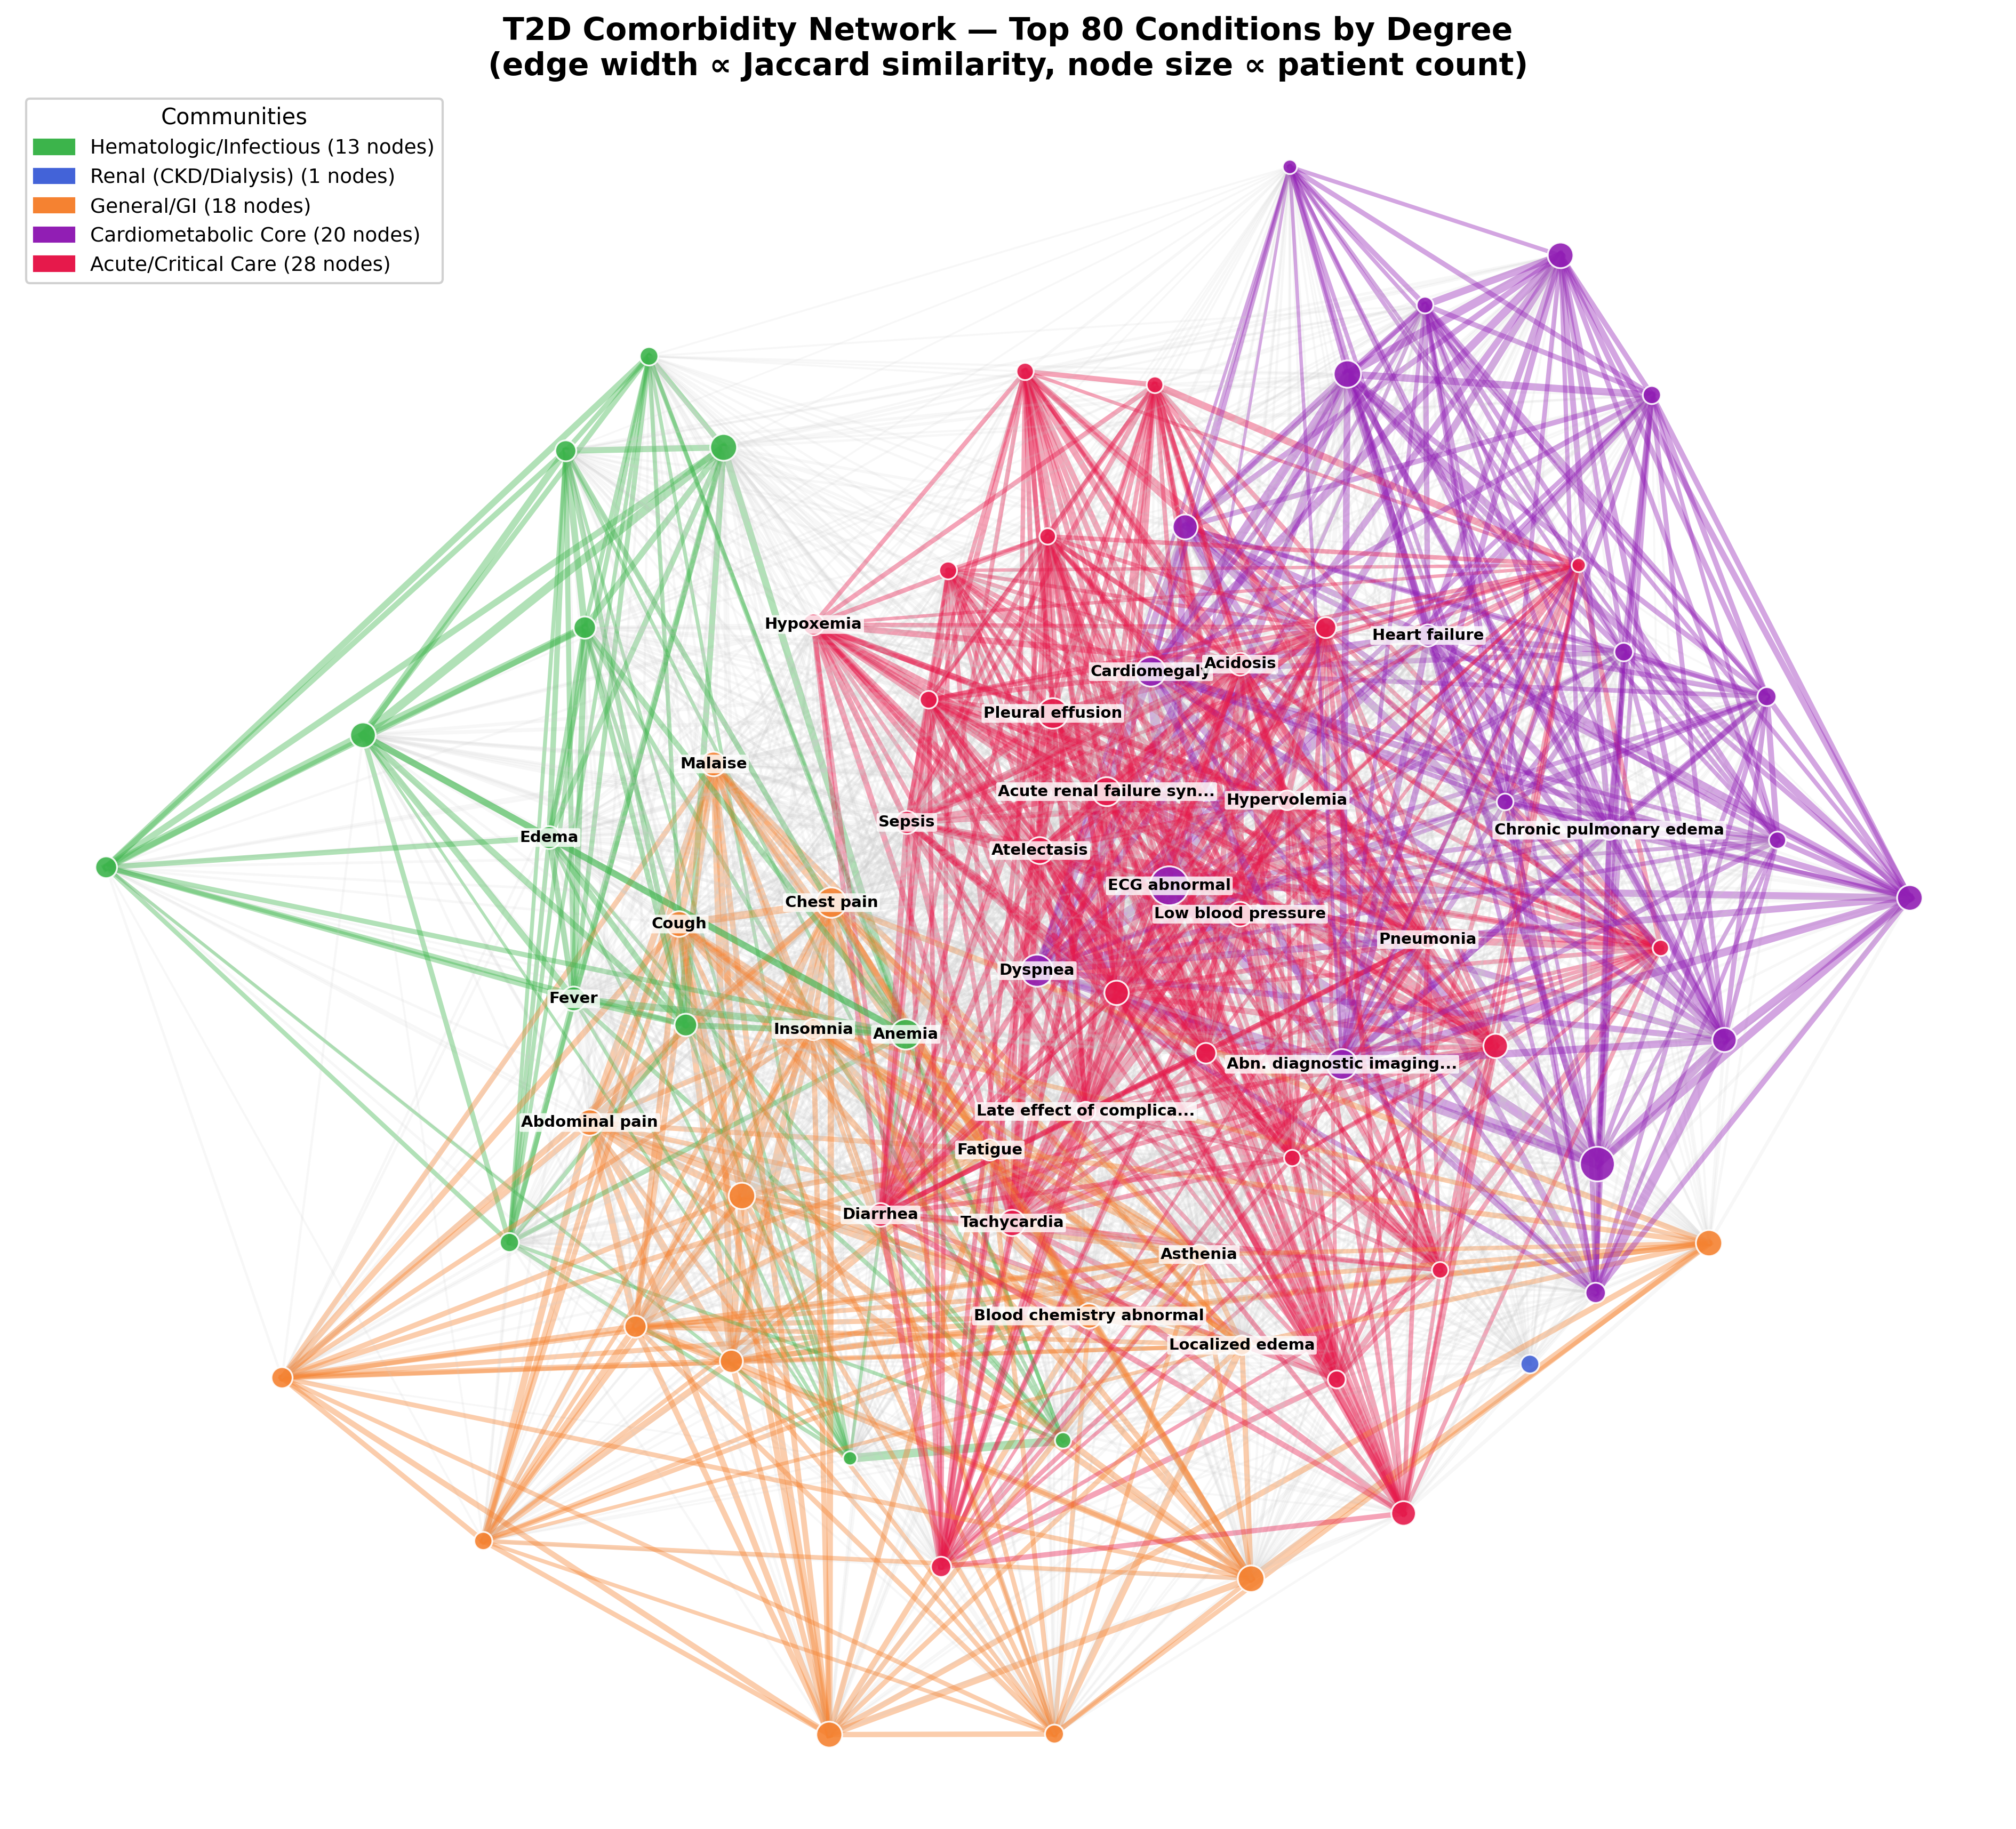
\includegraphics[width=\columnwidth]{figures/fig1_network_overview.png}
\caption{T2D comorbidity network (top 80 conditions by degree) colored by Louvain community. Edge width is proportional to Jaccard similarity; node size is proportional to patient count. Communities are visually separable: Cardiometabolic Core (purple), Acute/Critical Care (red), General/GI (orange), and Hematologic/Infectious (green).}
\label{fig:network}
\end{figure}

\begin{figure}[!htbp]
\centering
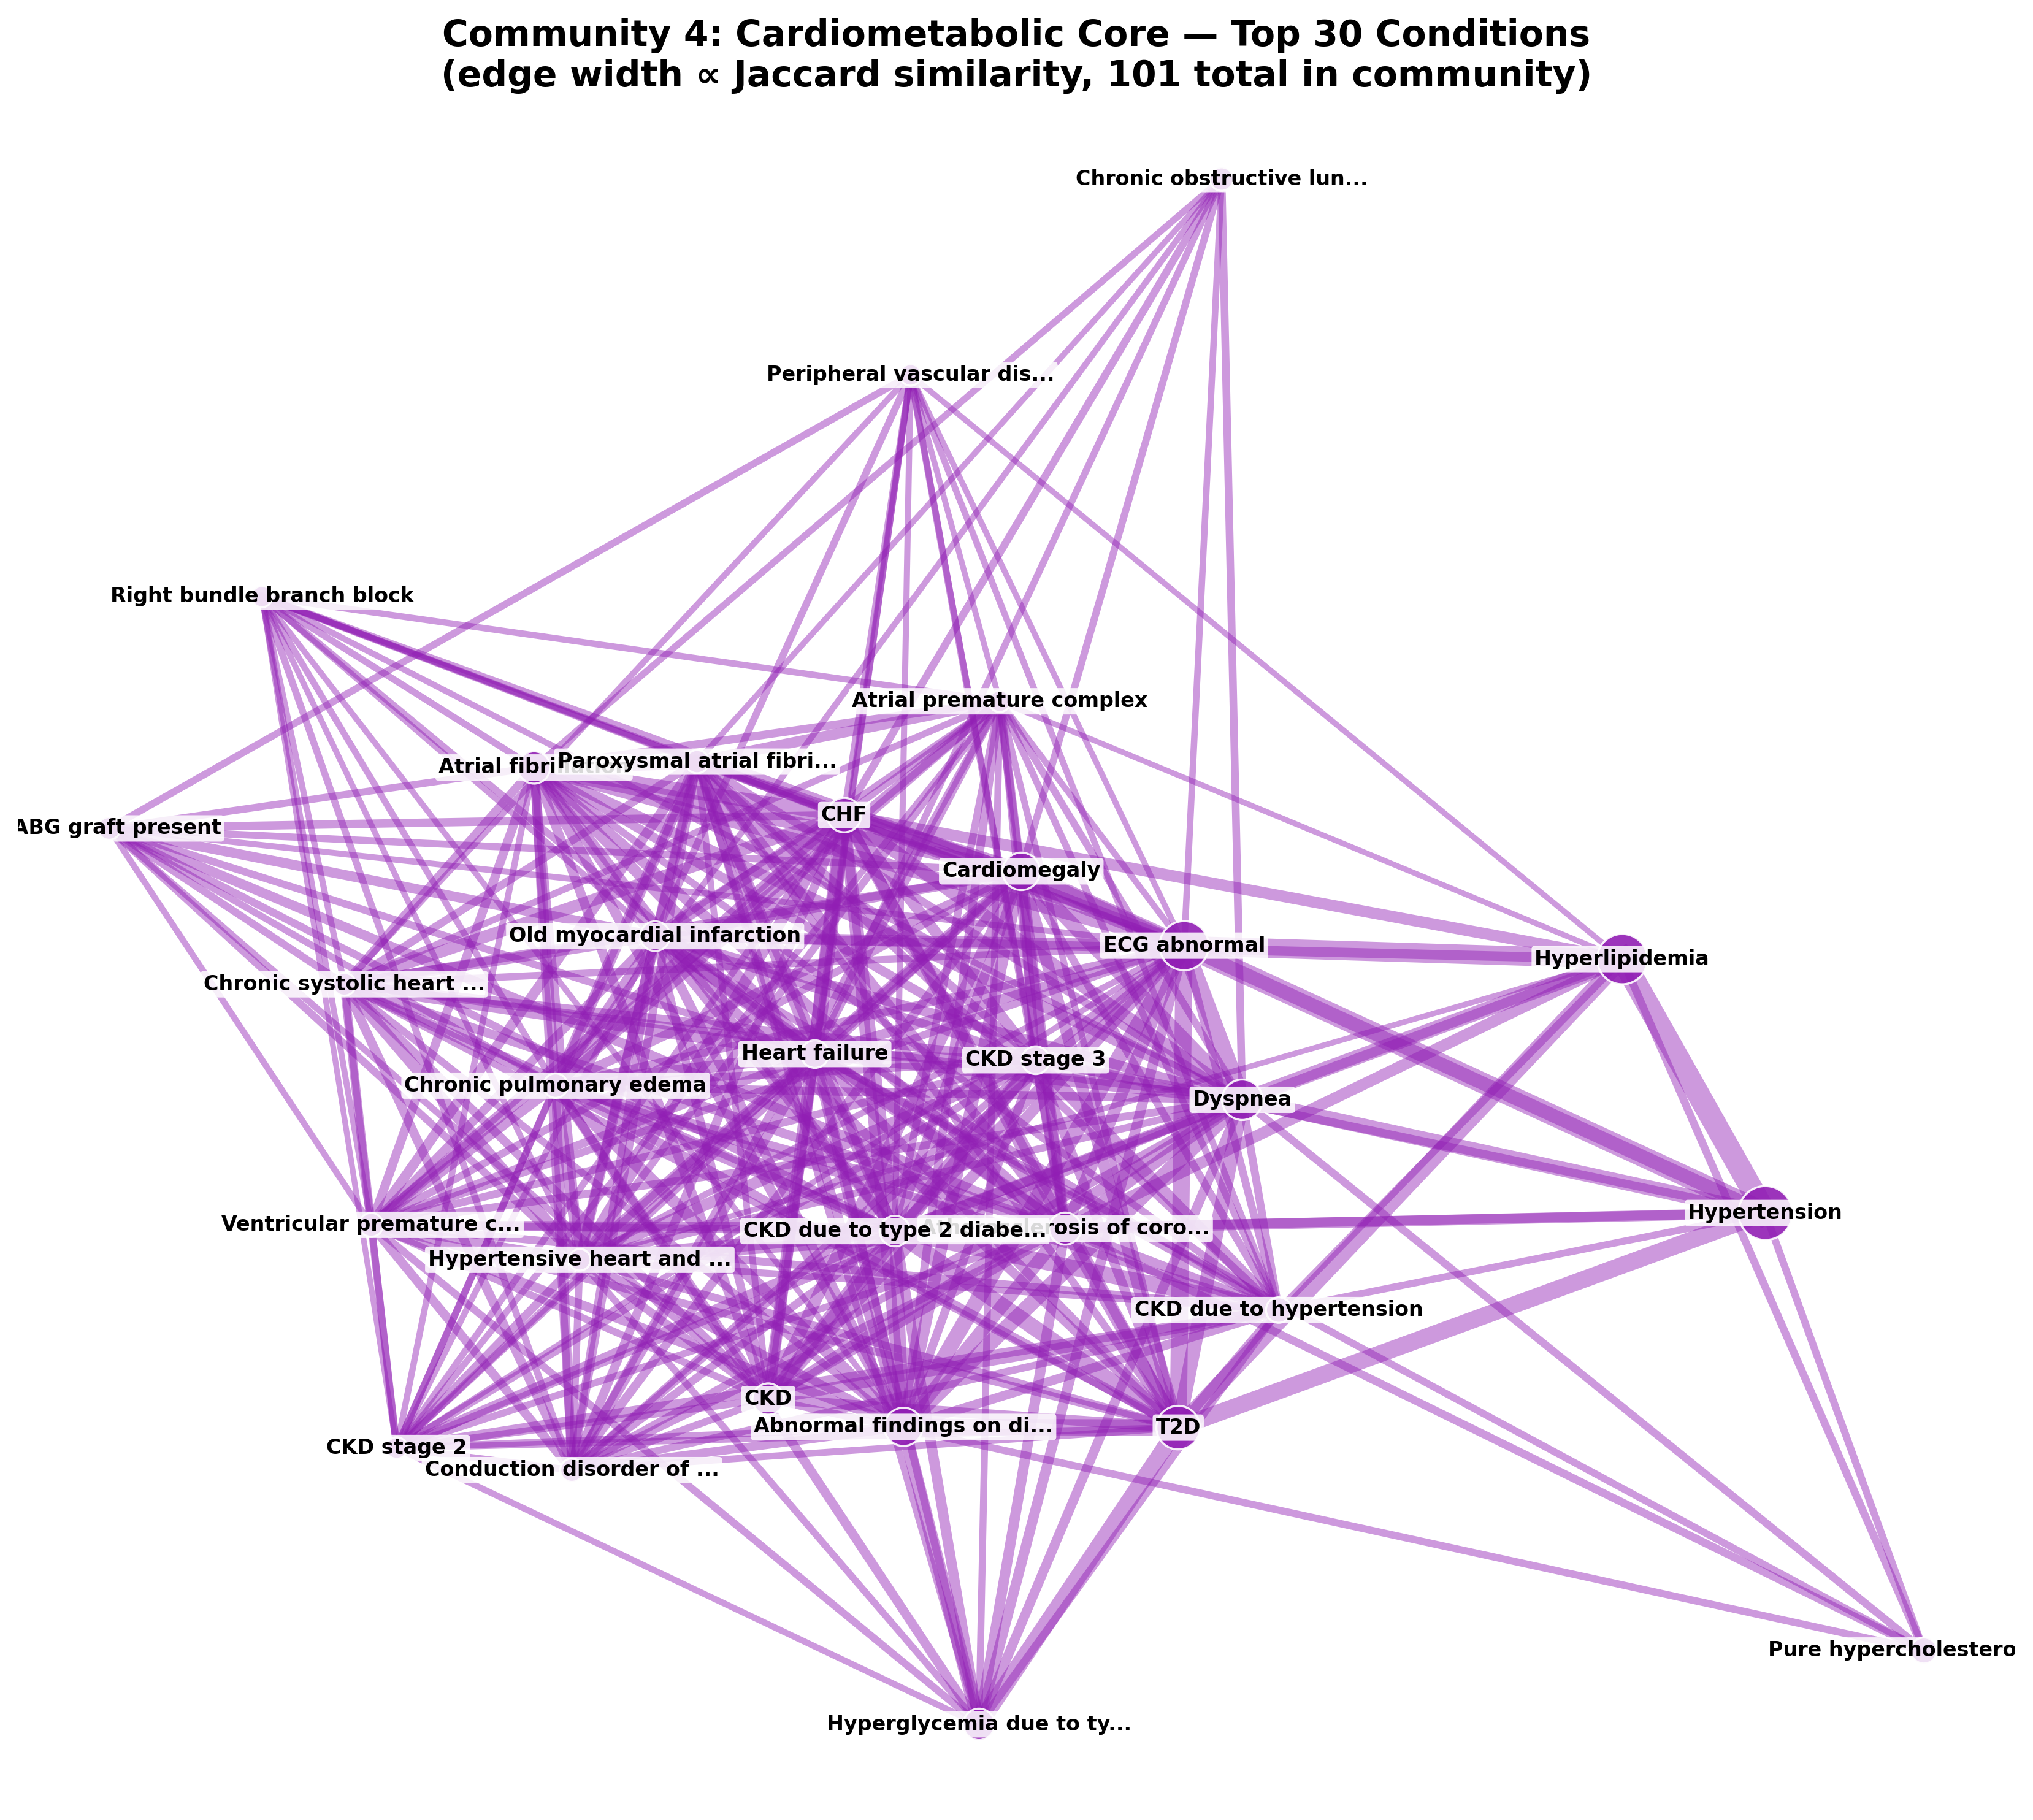
\includegraphics[width=\columnwidth]{figures/fig1b_community_zoomin.png}
\caption{Zoom-in on Community~4 (Cardiometabolic Core): top 30 conditions by patient count. Thicker edges indicate stronger Jaccard similarity. Hypertension, hyperlipidemia, T2D, and ECG abnormal form the densely connected center of this cluster, with CKD stages and heart failure conditions on the periphery.}
\label{fig:zoomin}
\end{figure}

\begin{figure}[!htbp]
\centering
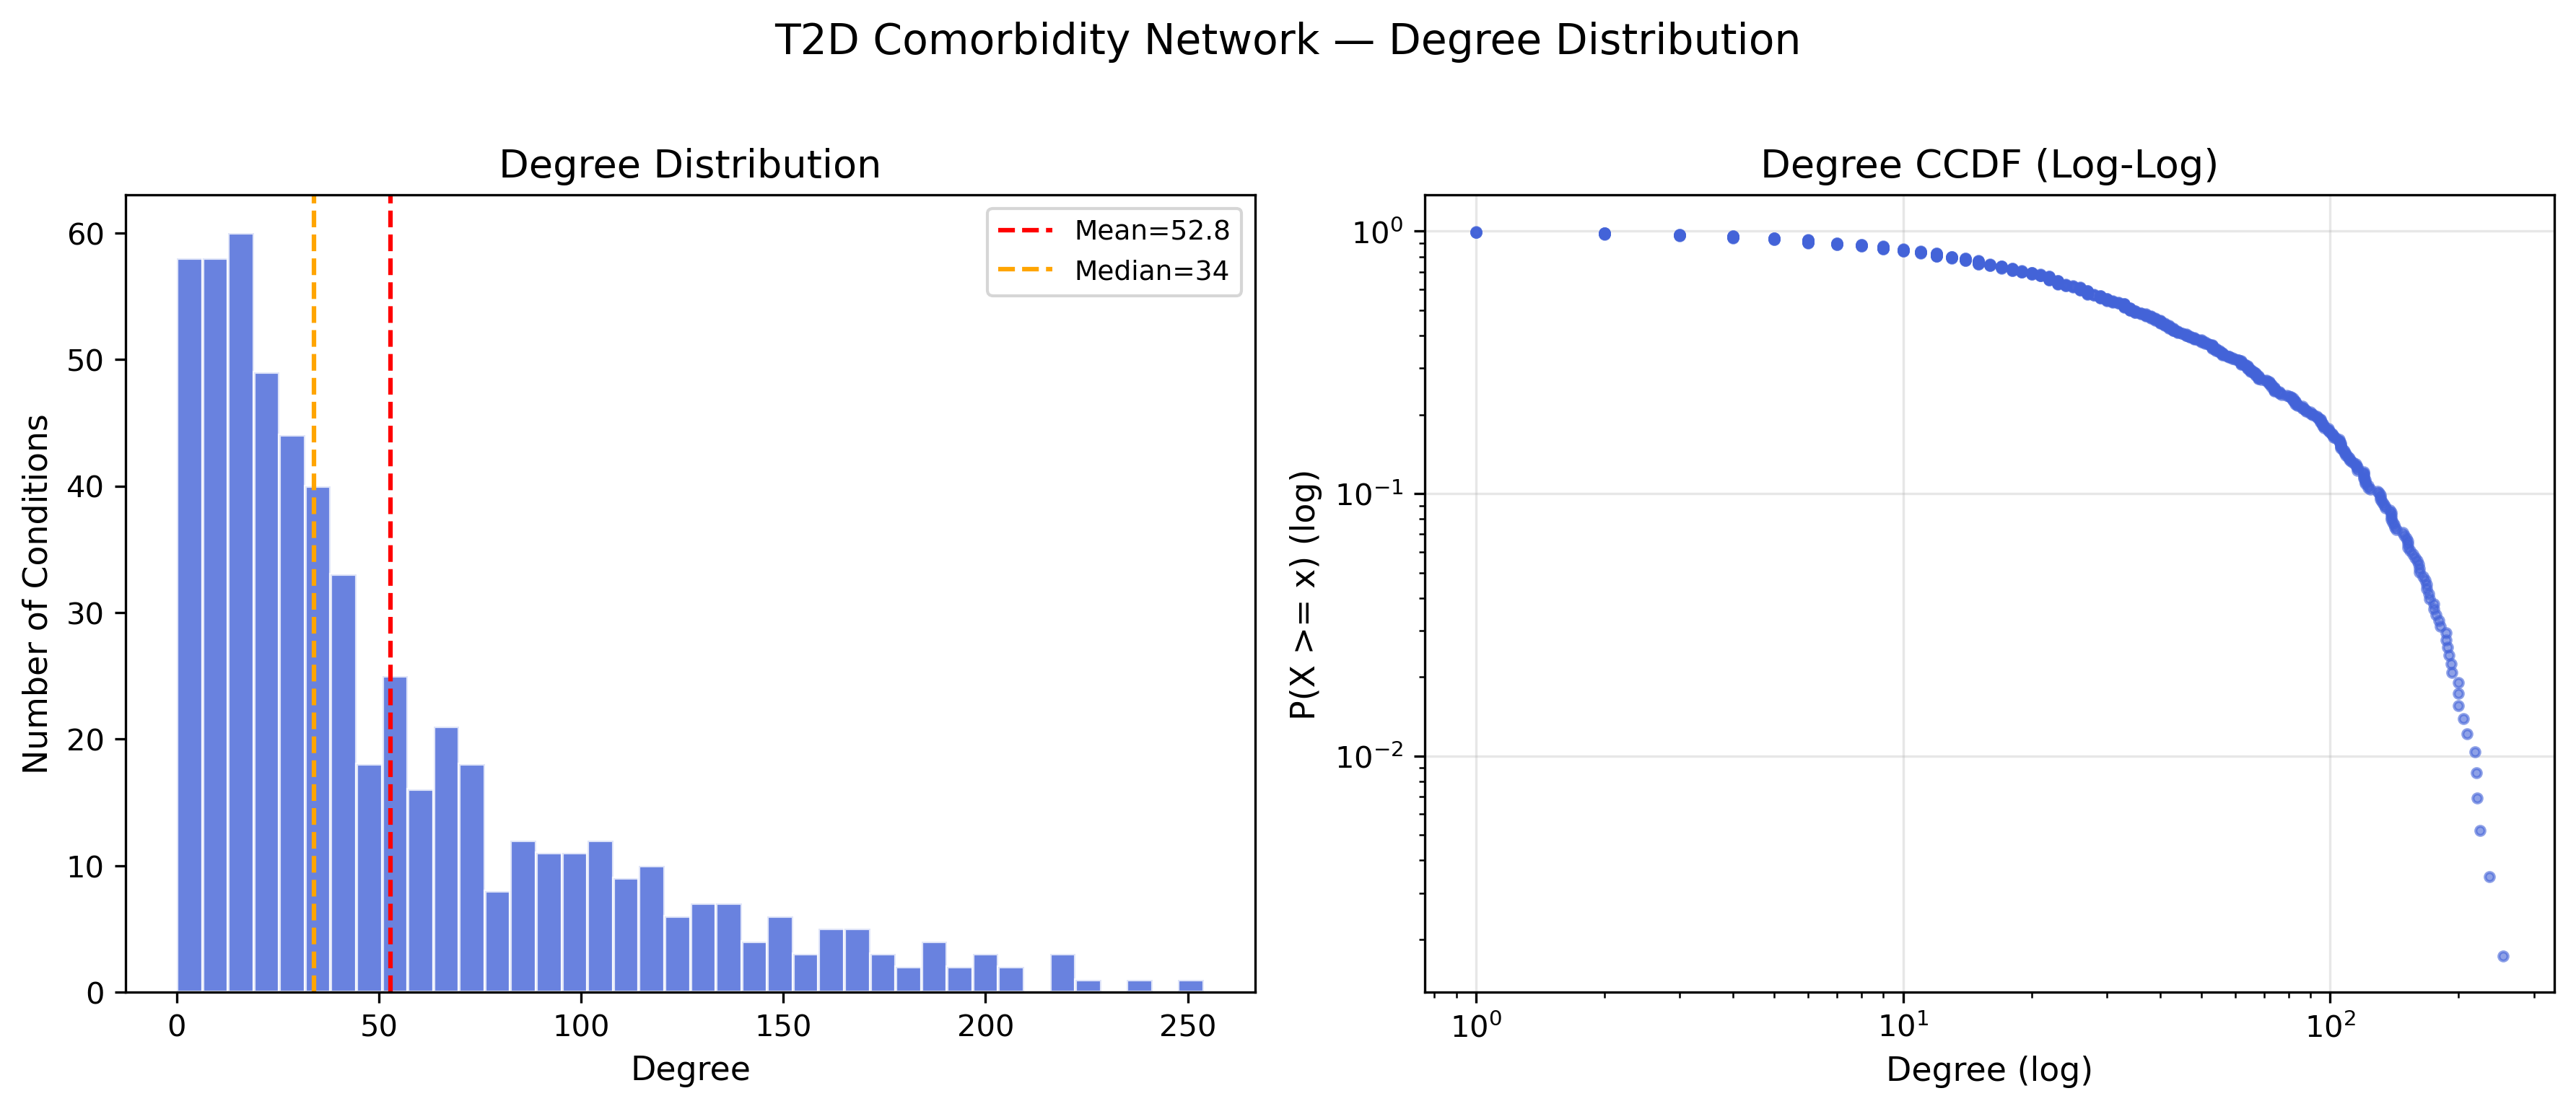
\includegraphics[width=\columnwidth]{figures/fig2_degree_distribution.png}
\caption{Degree distribution: histogram (left) and complementary cumulative distribution on log-log axes (right). The right-skewed distribution indicates a small number of hub conditions.}
\label{fig:degree}
\end{figure}

\begin{figure}[!htbp]
\centering
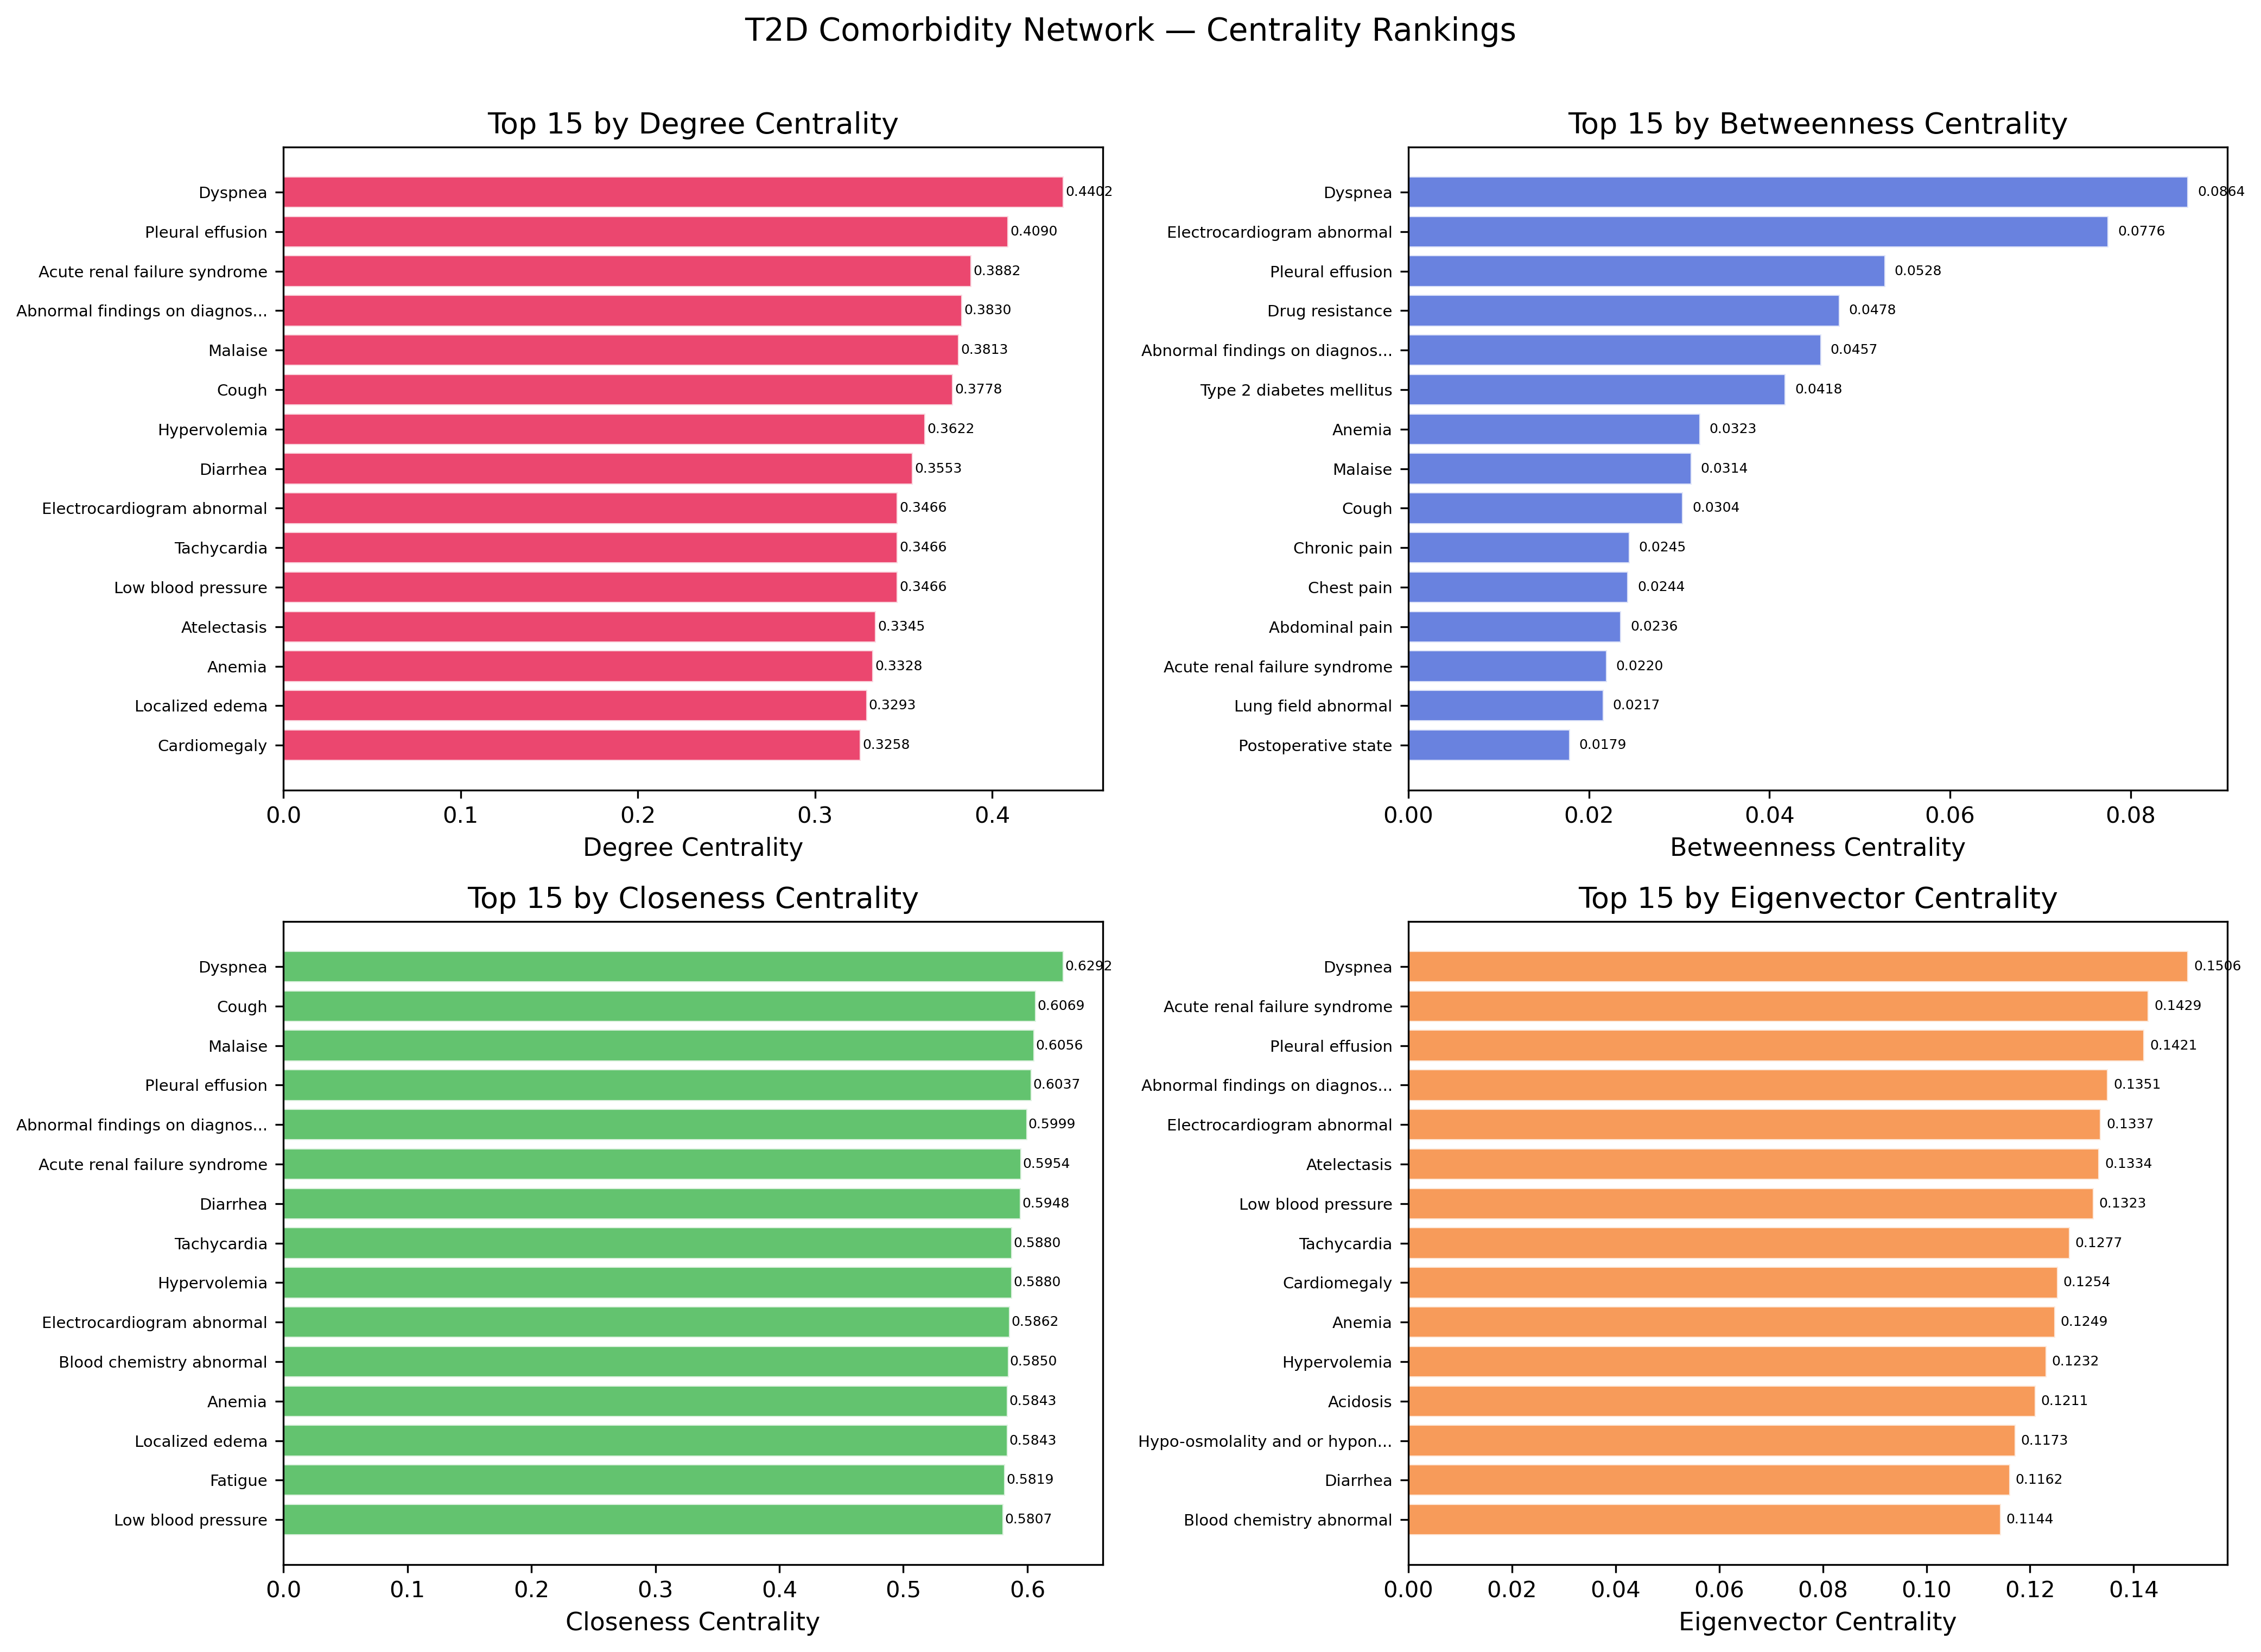
\includegraphics[width=\columnwidth]{figures/fig3_centrality_rankings.png}
\caption{Top 15 conditions ranked by four centrality measures: degree, betweenness, closeness, and eigenvector. Dyspnea ranks first across all four, confirming its role as the network's primary hub.}
\label{fig:centrality}
\end{figure}

\begin{figure}[!htbp]
\centering
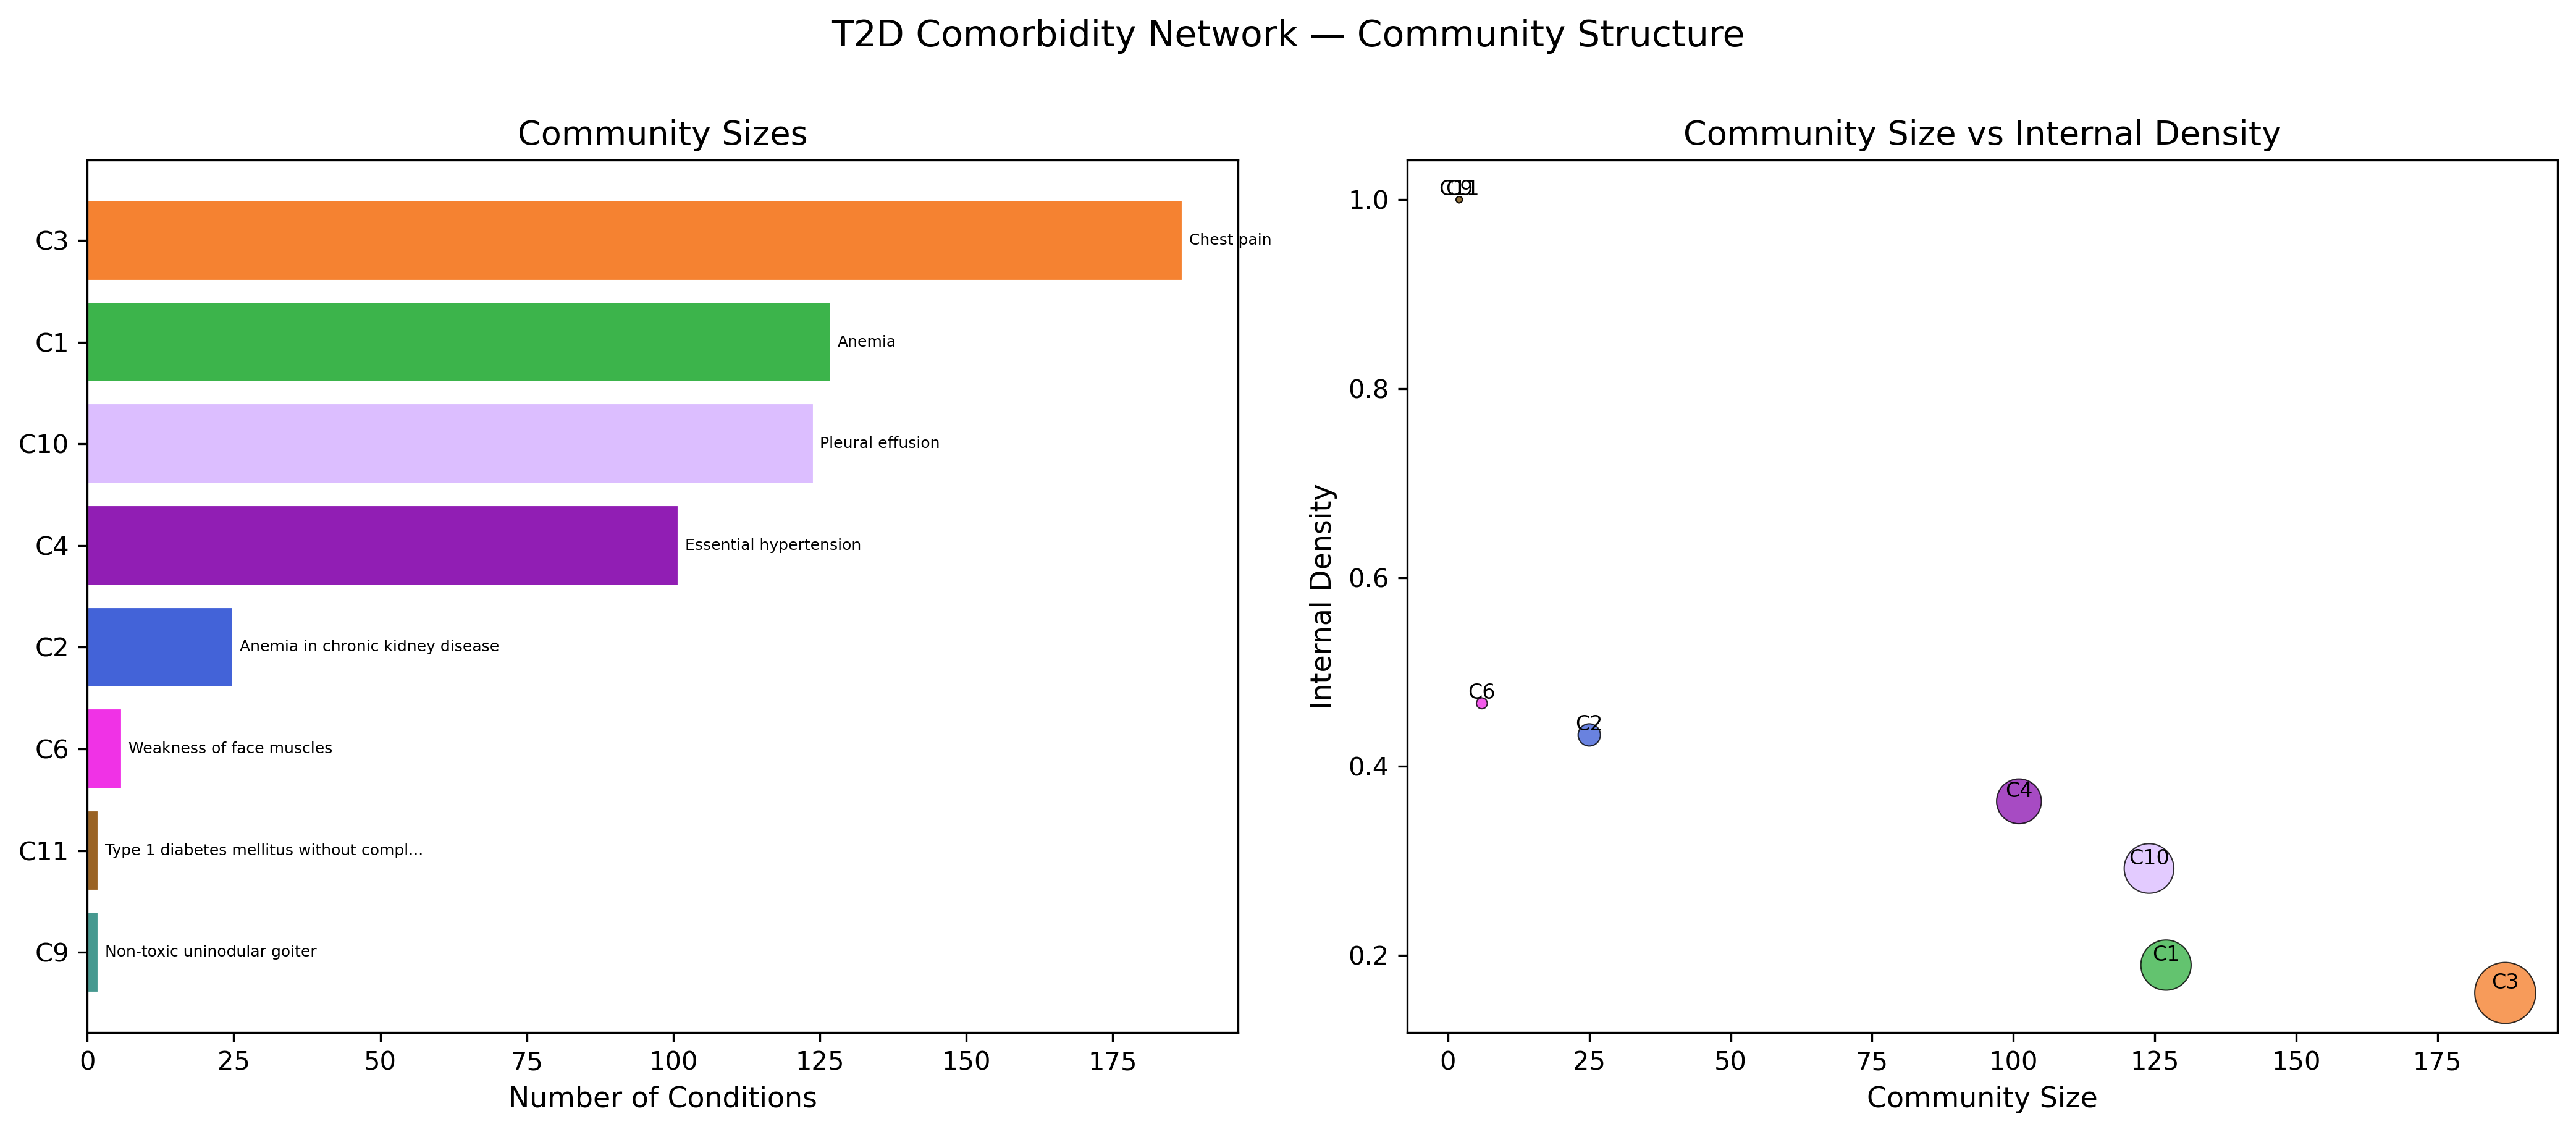
\includegraphics[width=\columnwidth]{figures/fig4_community_composition.png}
\caption{Community structure: sizes of Louvain communities (left) and the relationship between community size and internal density (right). Smaller communities (C2, C6) are more internally dense than larger ones (C3, C1).}
\label{fig:communities}
\end{figure}

\begin{figure}[!htbp]
\centering
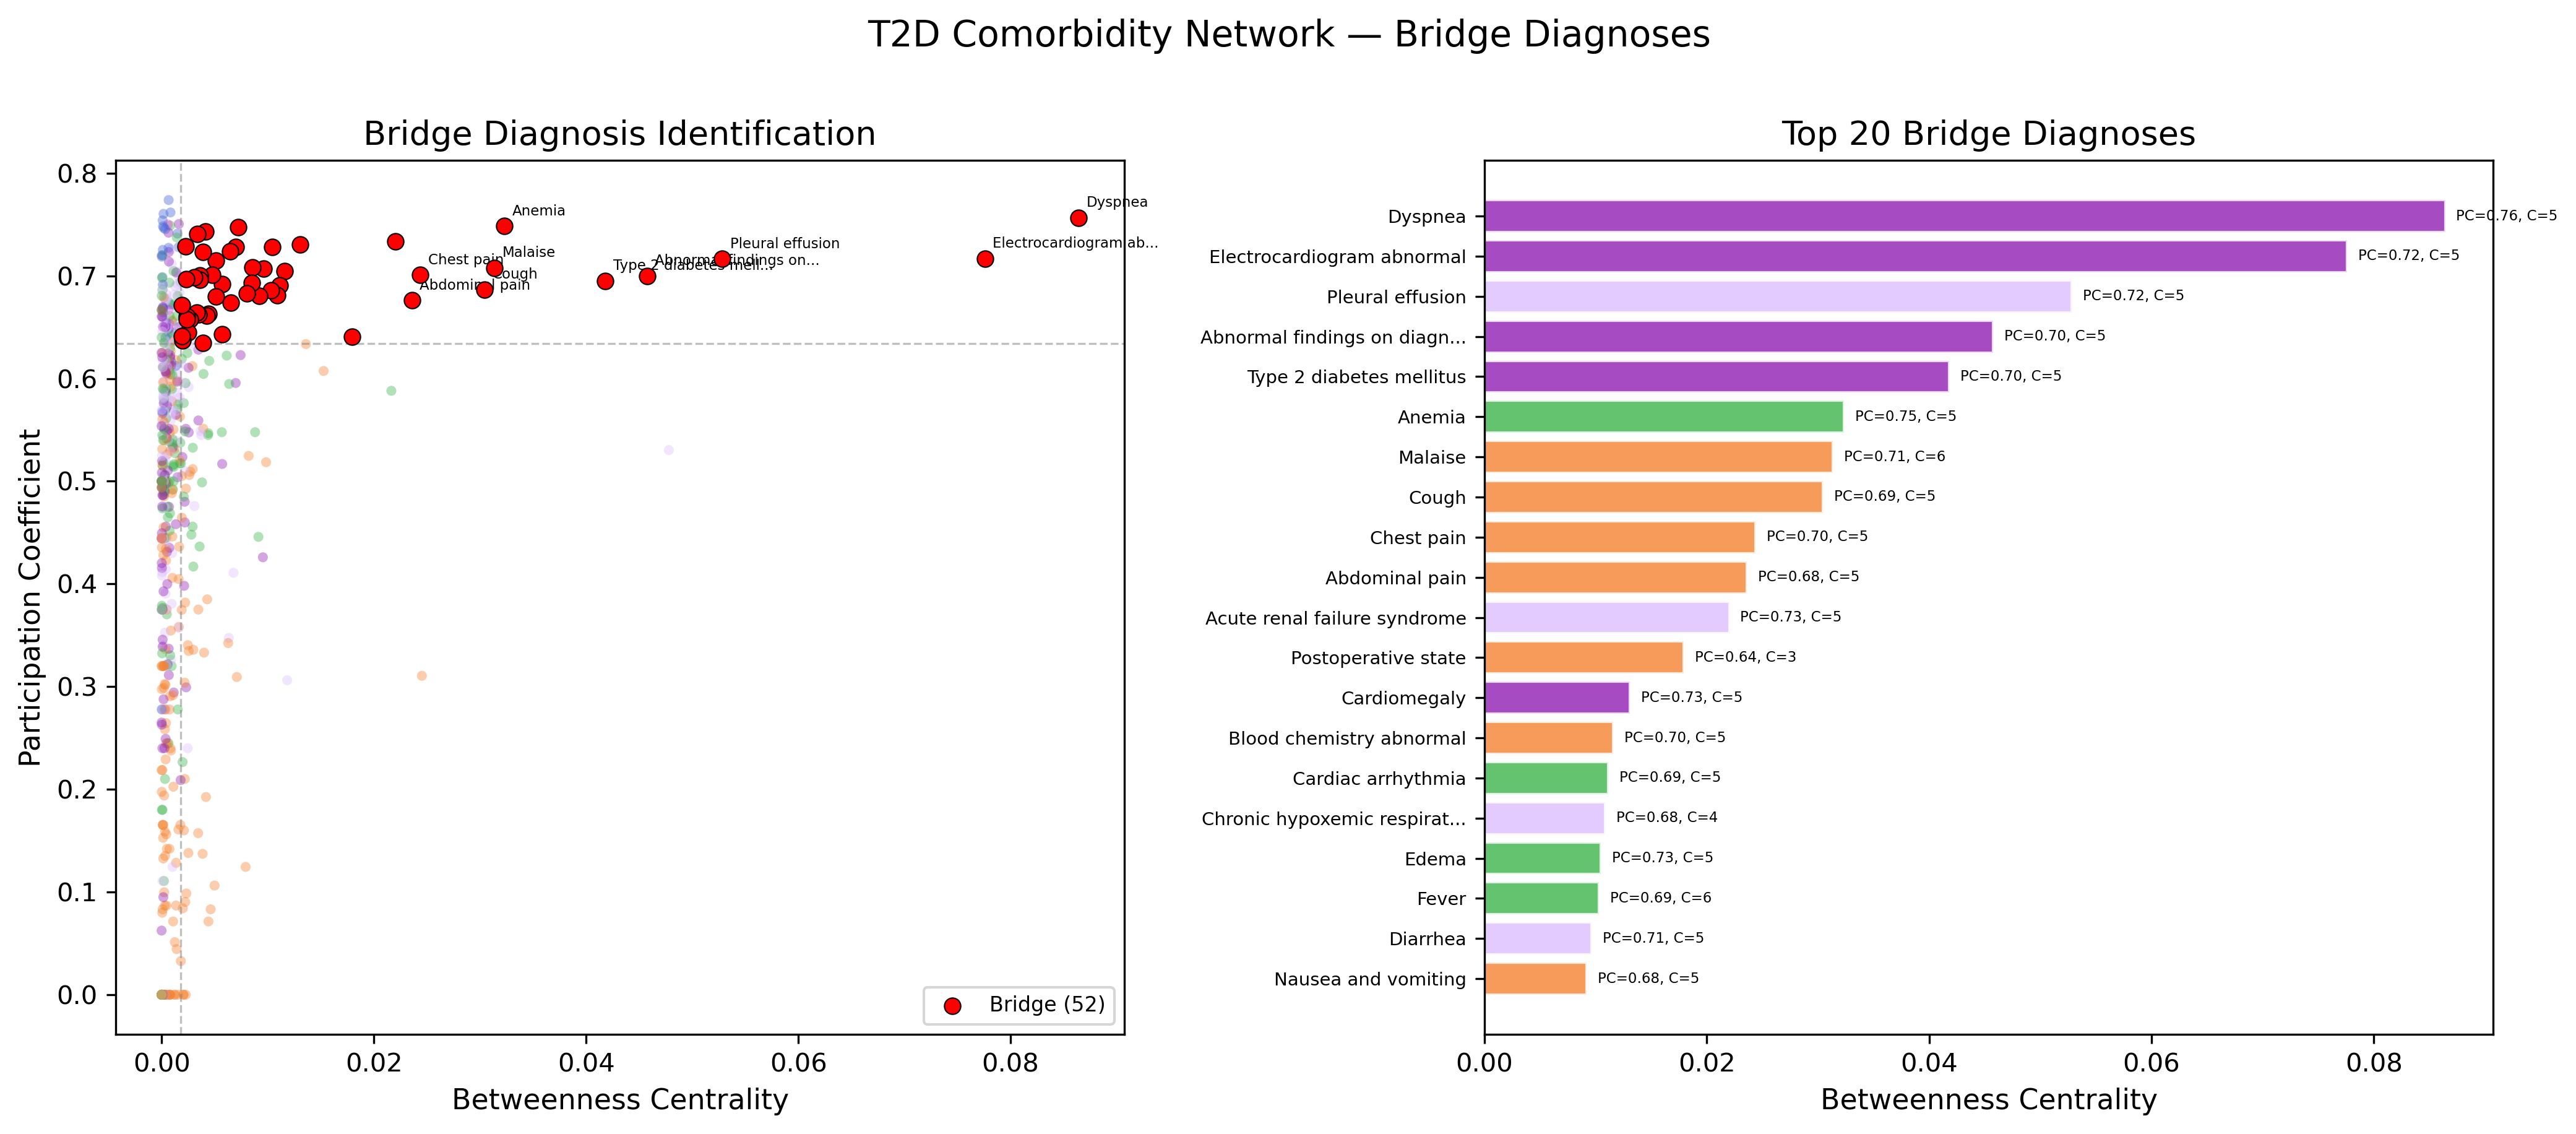
\includegraphics[width=\columnwidth]{figures/fig5_bridge_diagnoses.png}
\caption{Bridge diagnosis identification. Left: all conditions plotted by betweenness centrality vs.\ participation coefficient; red points in the upper-right quadrant are bridges. Right: top 20 bridges ranked by betweenness.}
\label{fig:bridges}
\end{figure}

\begin{figure}[!htbp]
\centering
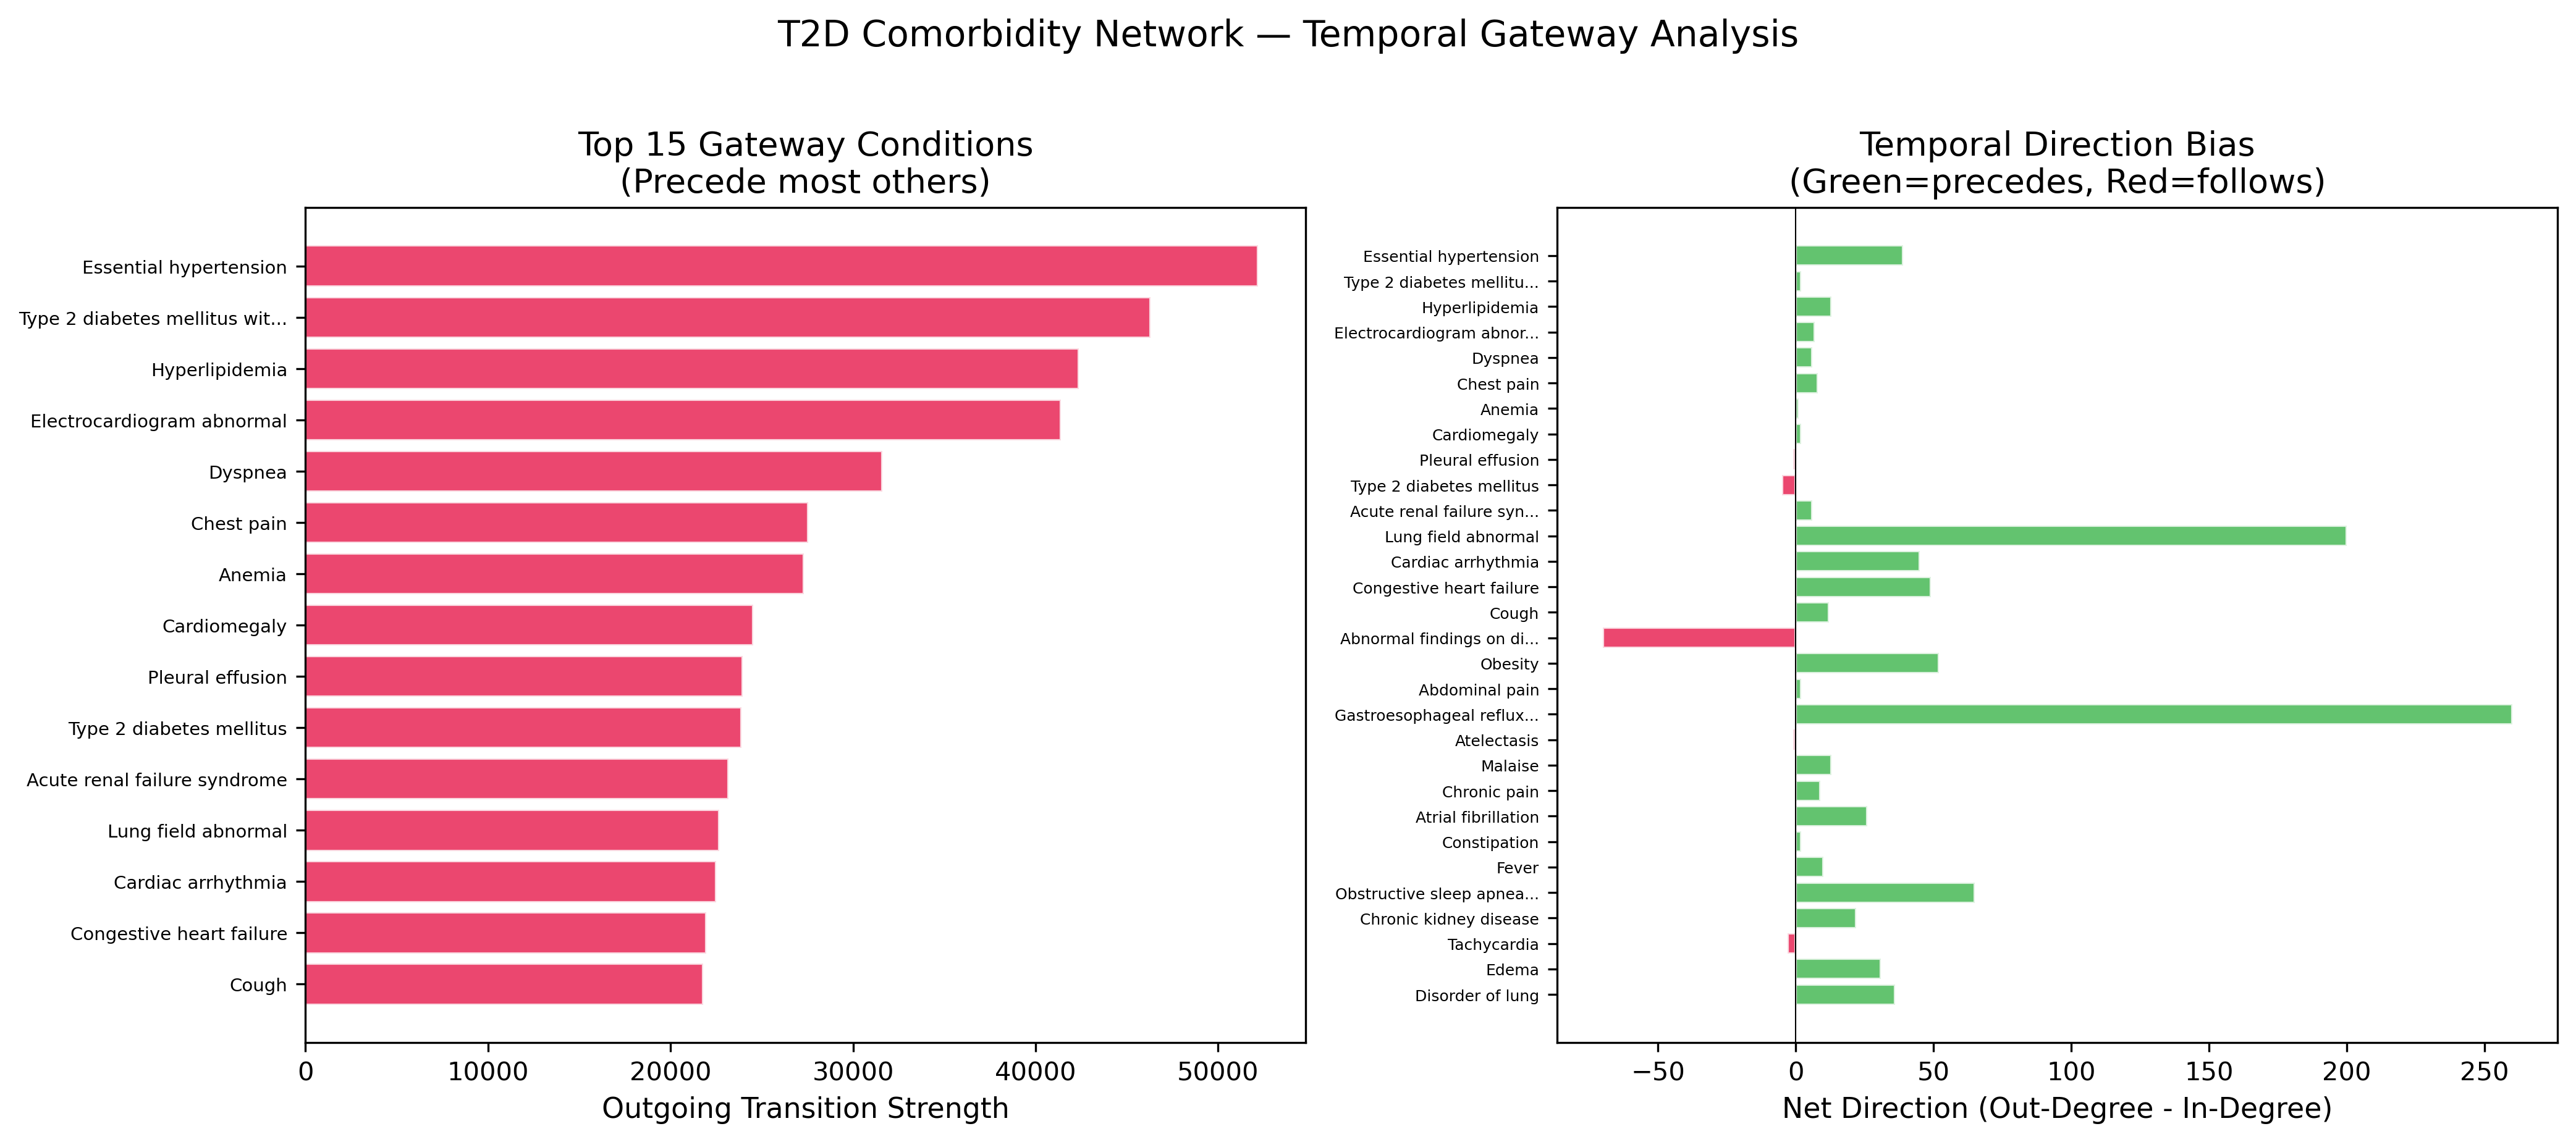
\includegraphics[width=\columnwidth]{figures/fig6_temporal_gateways.png}
\caption{Temporal gateway analysis. Left: top 15 conditions by outgoing transition strength. Right: net temporal direction bias---green bars indicate conditions that precede others; red bars indicate conditions that follow.}
\label{fig:temporal}
\end{figure}

\begin{figure}[!htbp]
\centering
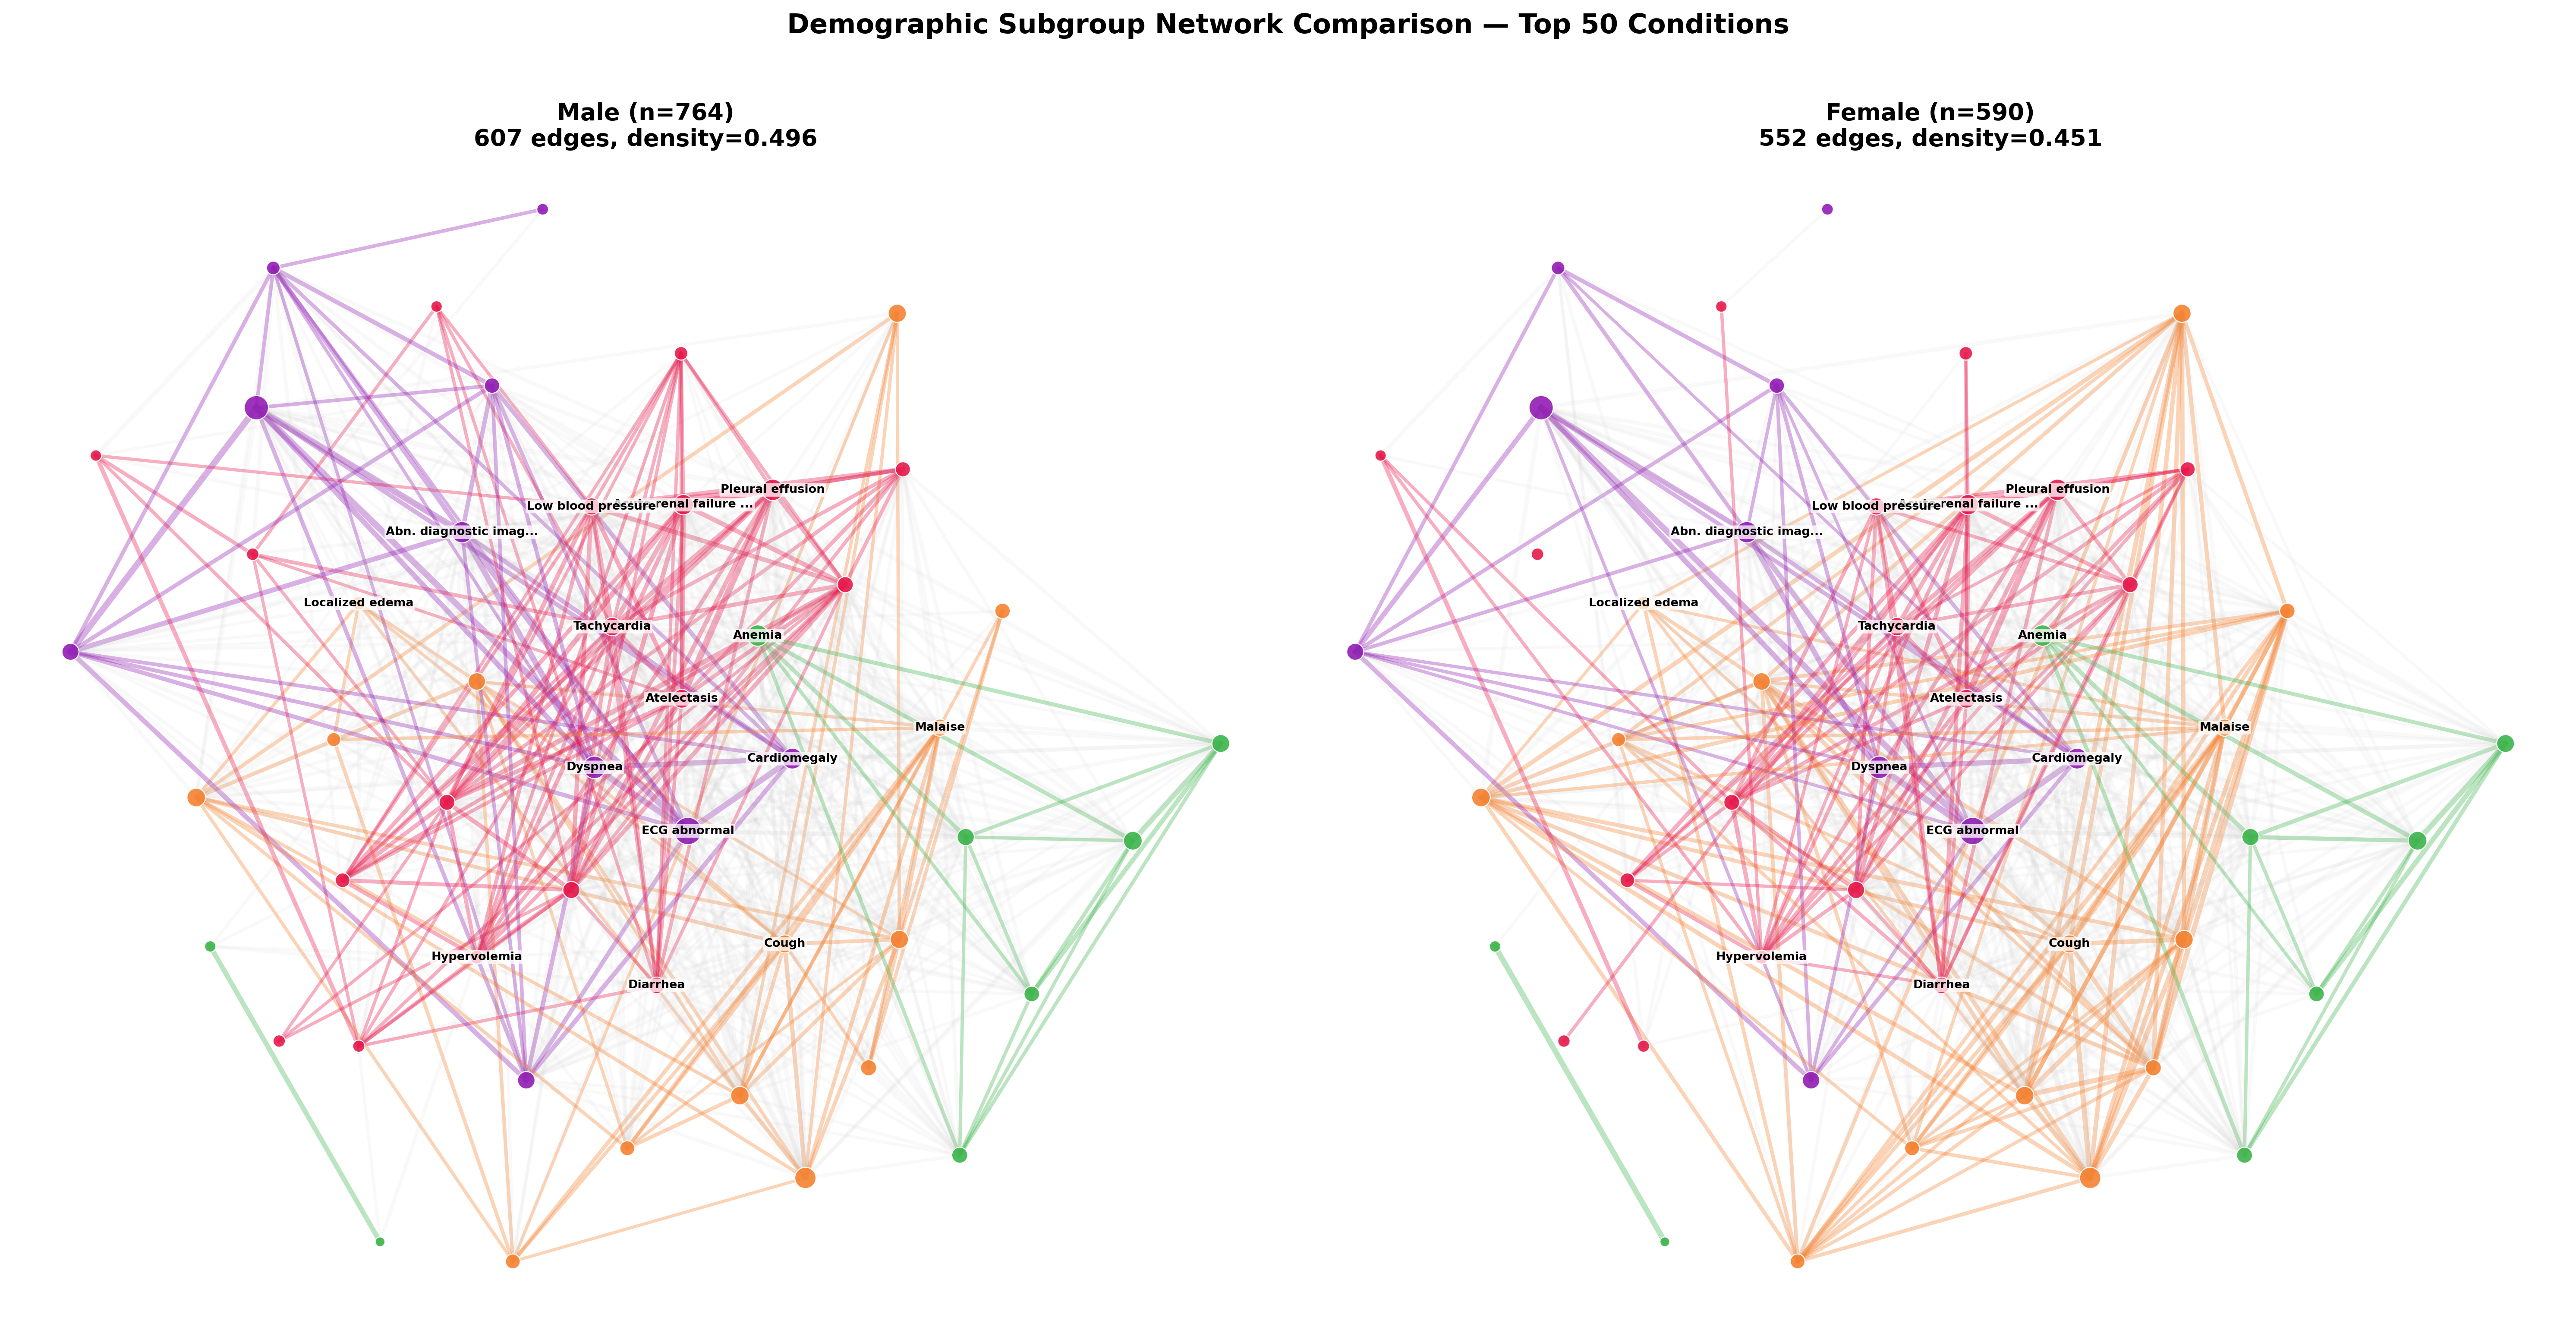
\includegraphics[width=\columnwidth]{figures/fig1c_subgroup_networks.png}
\caption{Side-by-side network comparison of top 50 conditions in Male (n=764) vs.\ Female (n=590) subgroups (edges with Jaccard $\geq$ 0.25 shown). Male patients show higher density (0.496 vs.\ 0.451), indicating more widespread co-occurrence of conditions.}
\label{fig:subgroup_nets}
\end{figure}

\begin{figure}[!htbp]
\centering
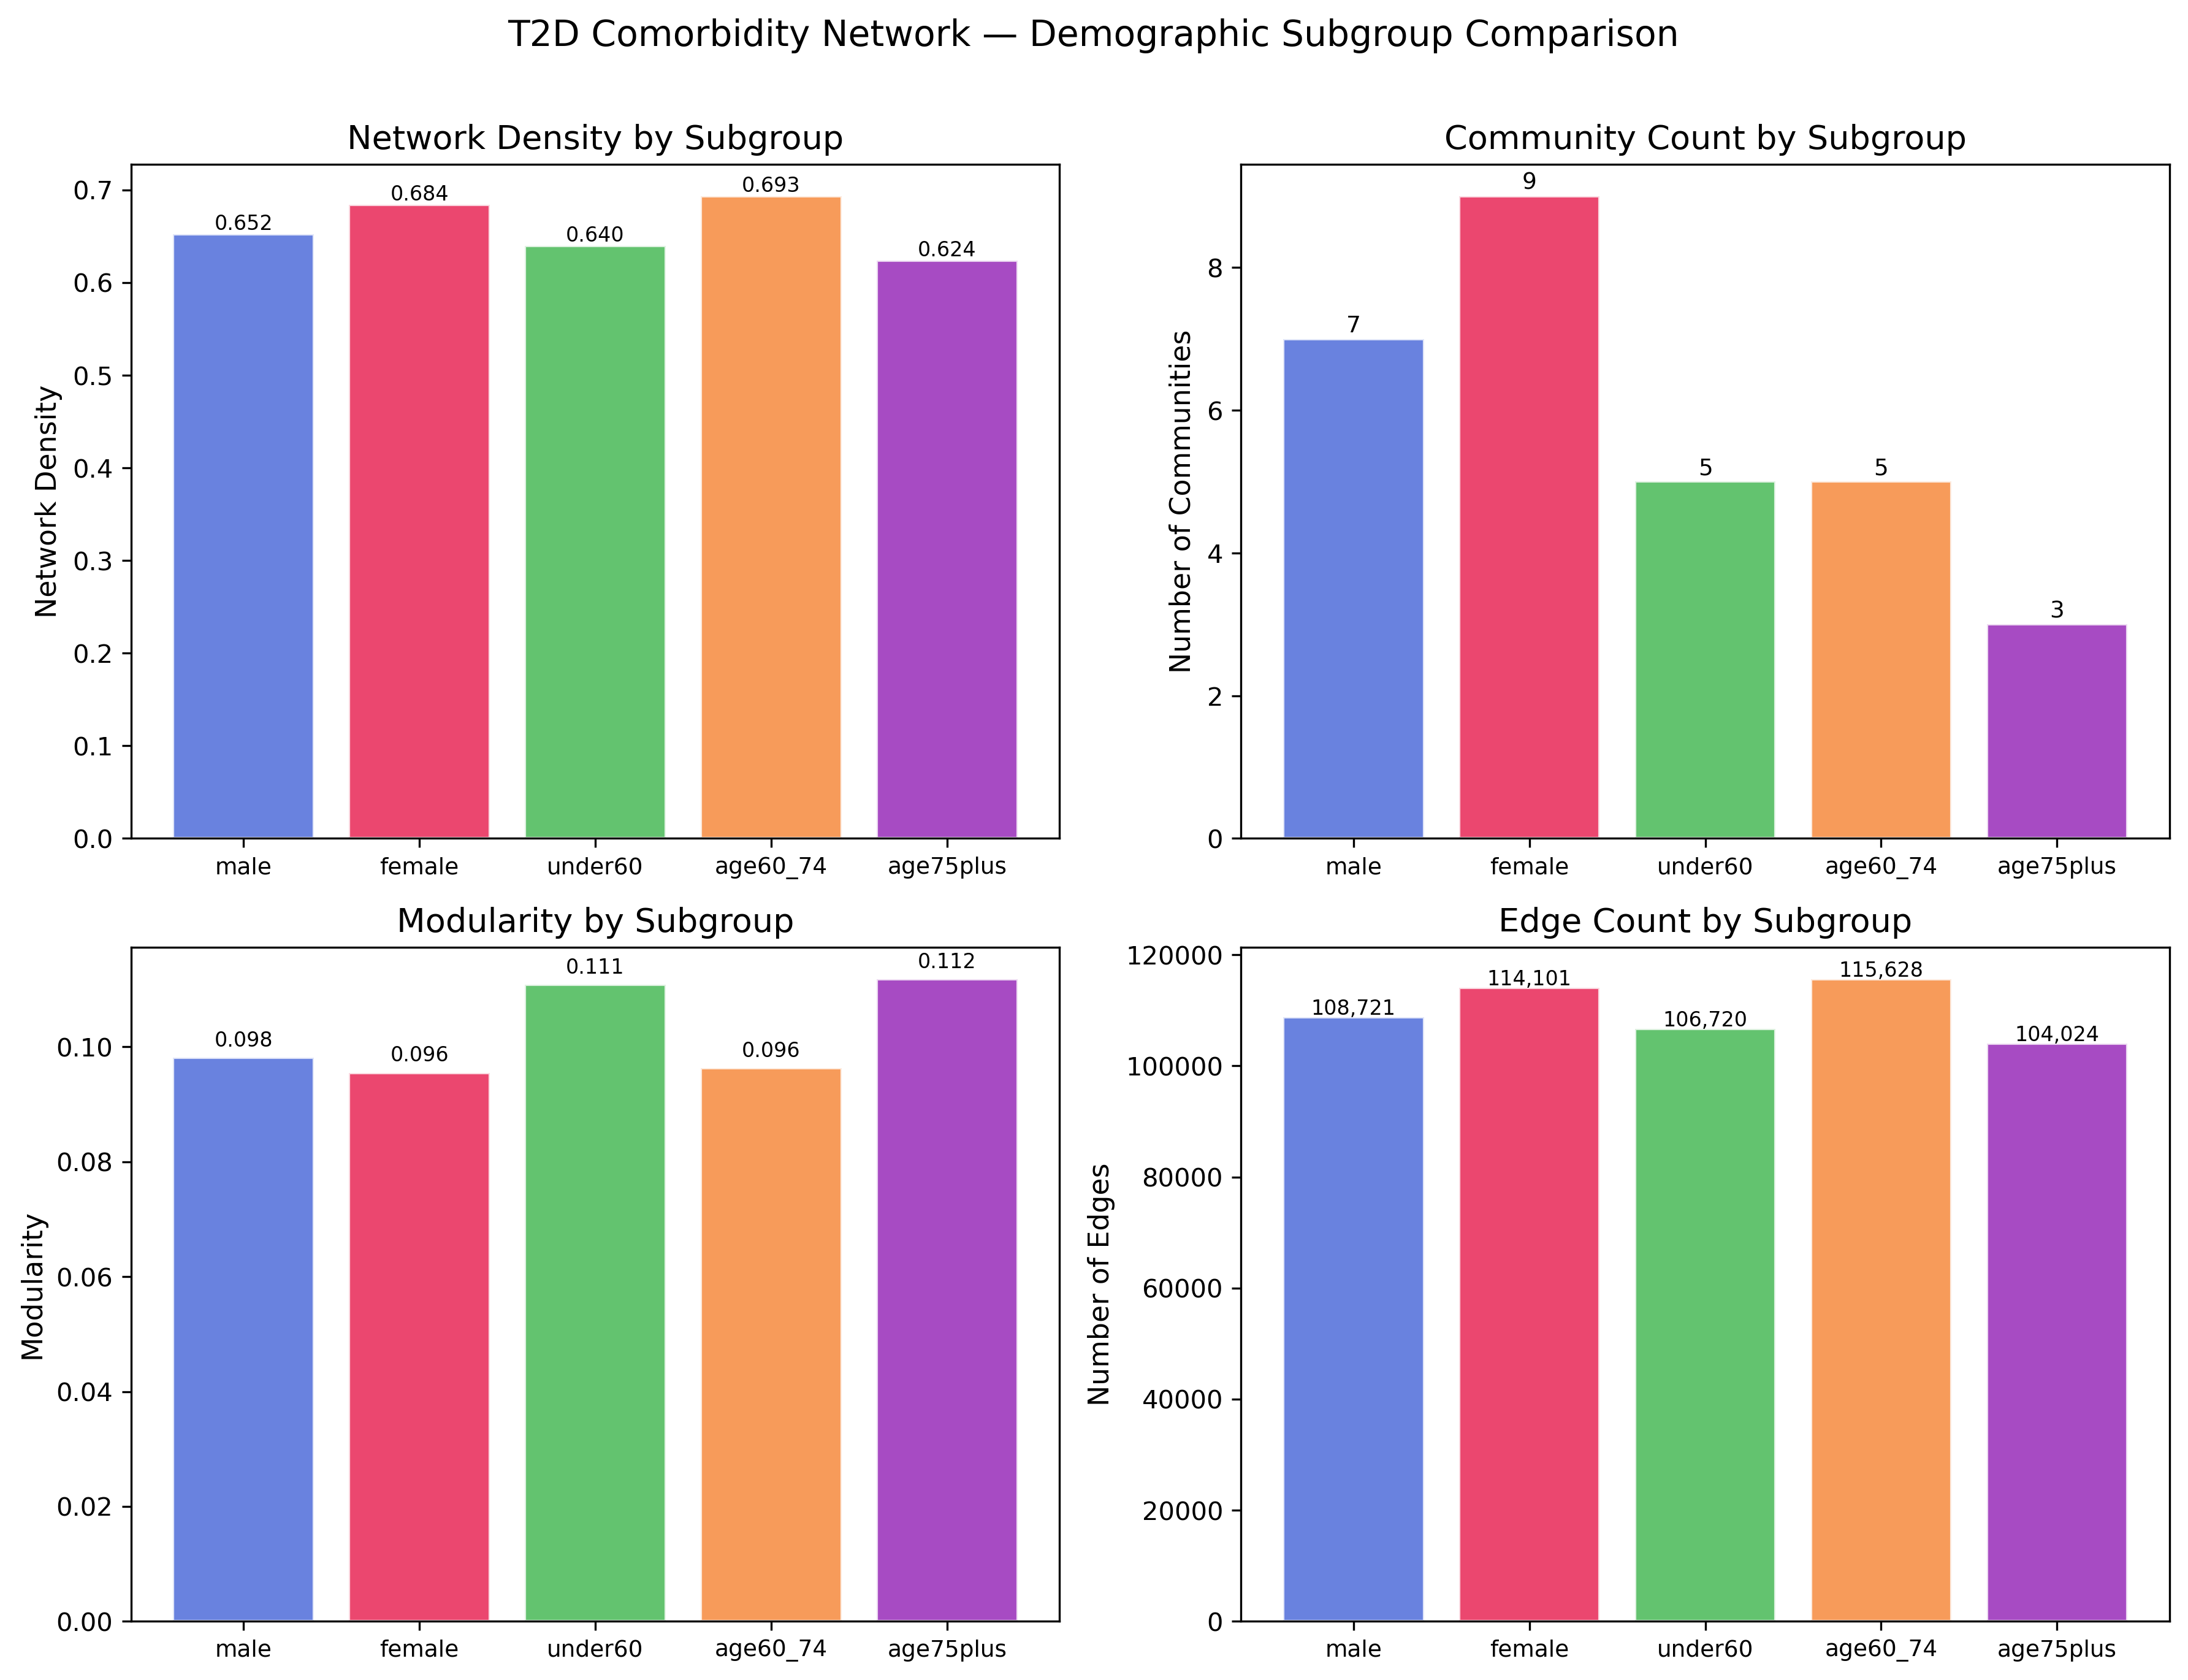
\includegraphics[width=\columnwidth]{figures/fig7_demographic_comparison.png}
\caption{Demographic subgroup comparison across density, community count, modularity, and edge count.}
\label{fig:demographics}
\end{figure}

\begin{figure}[!htbp]
\centering
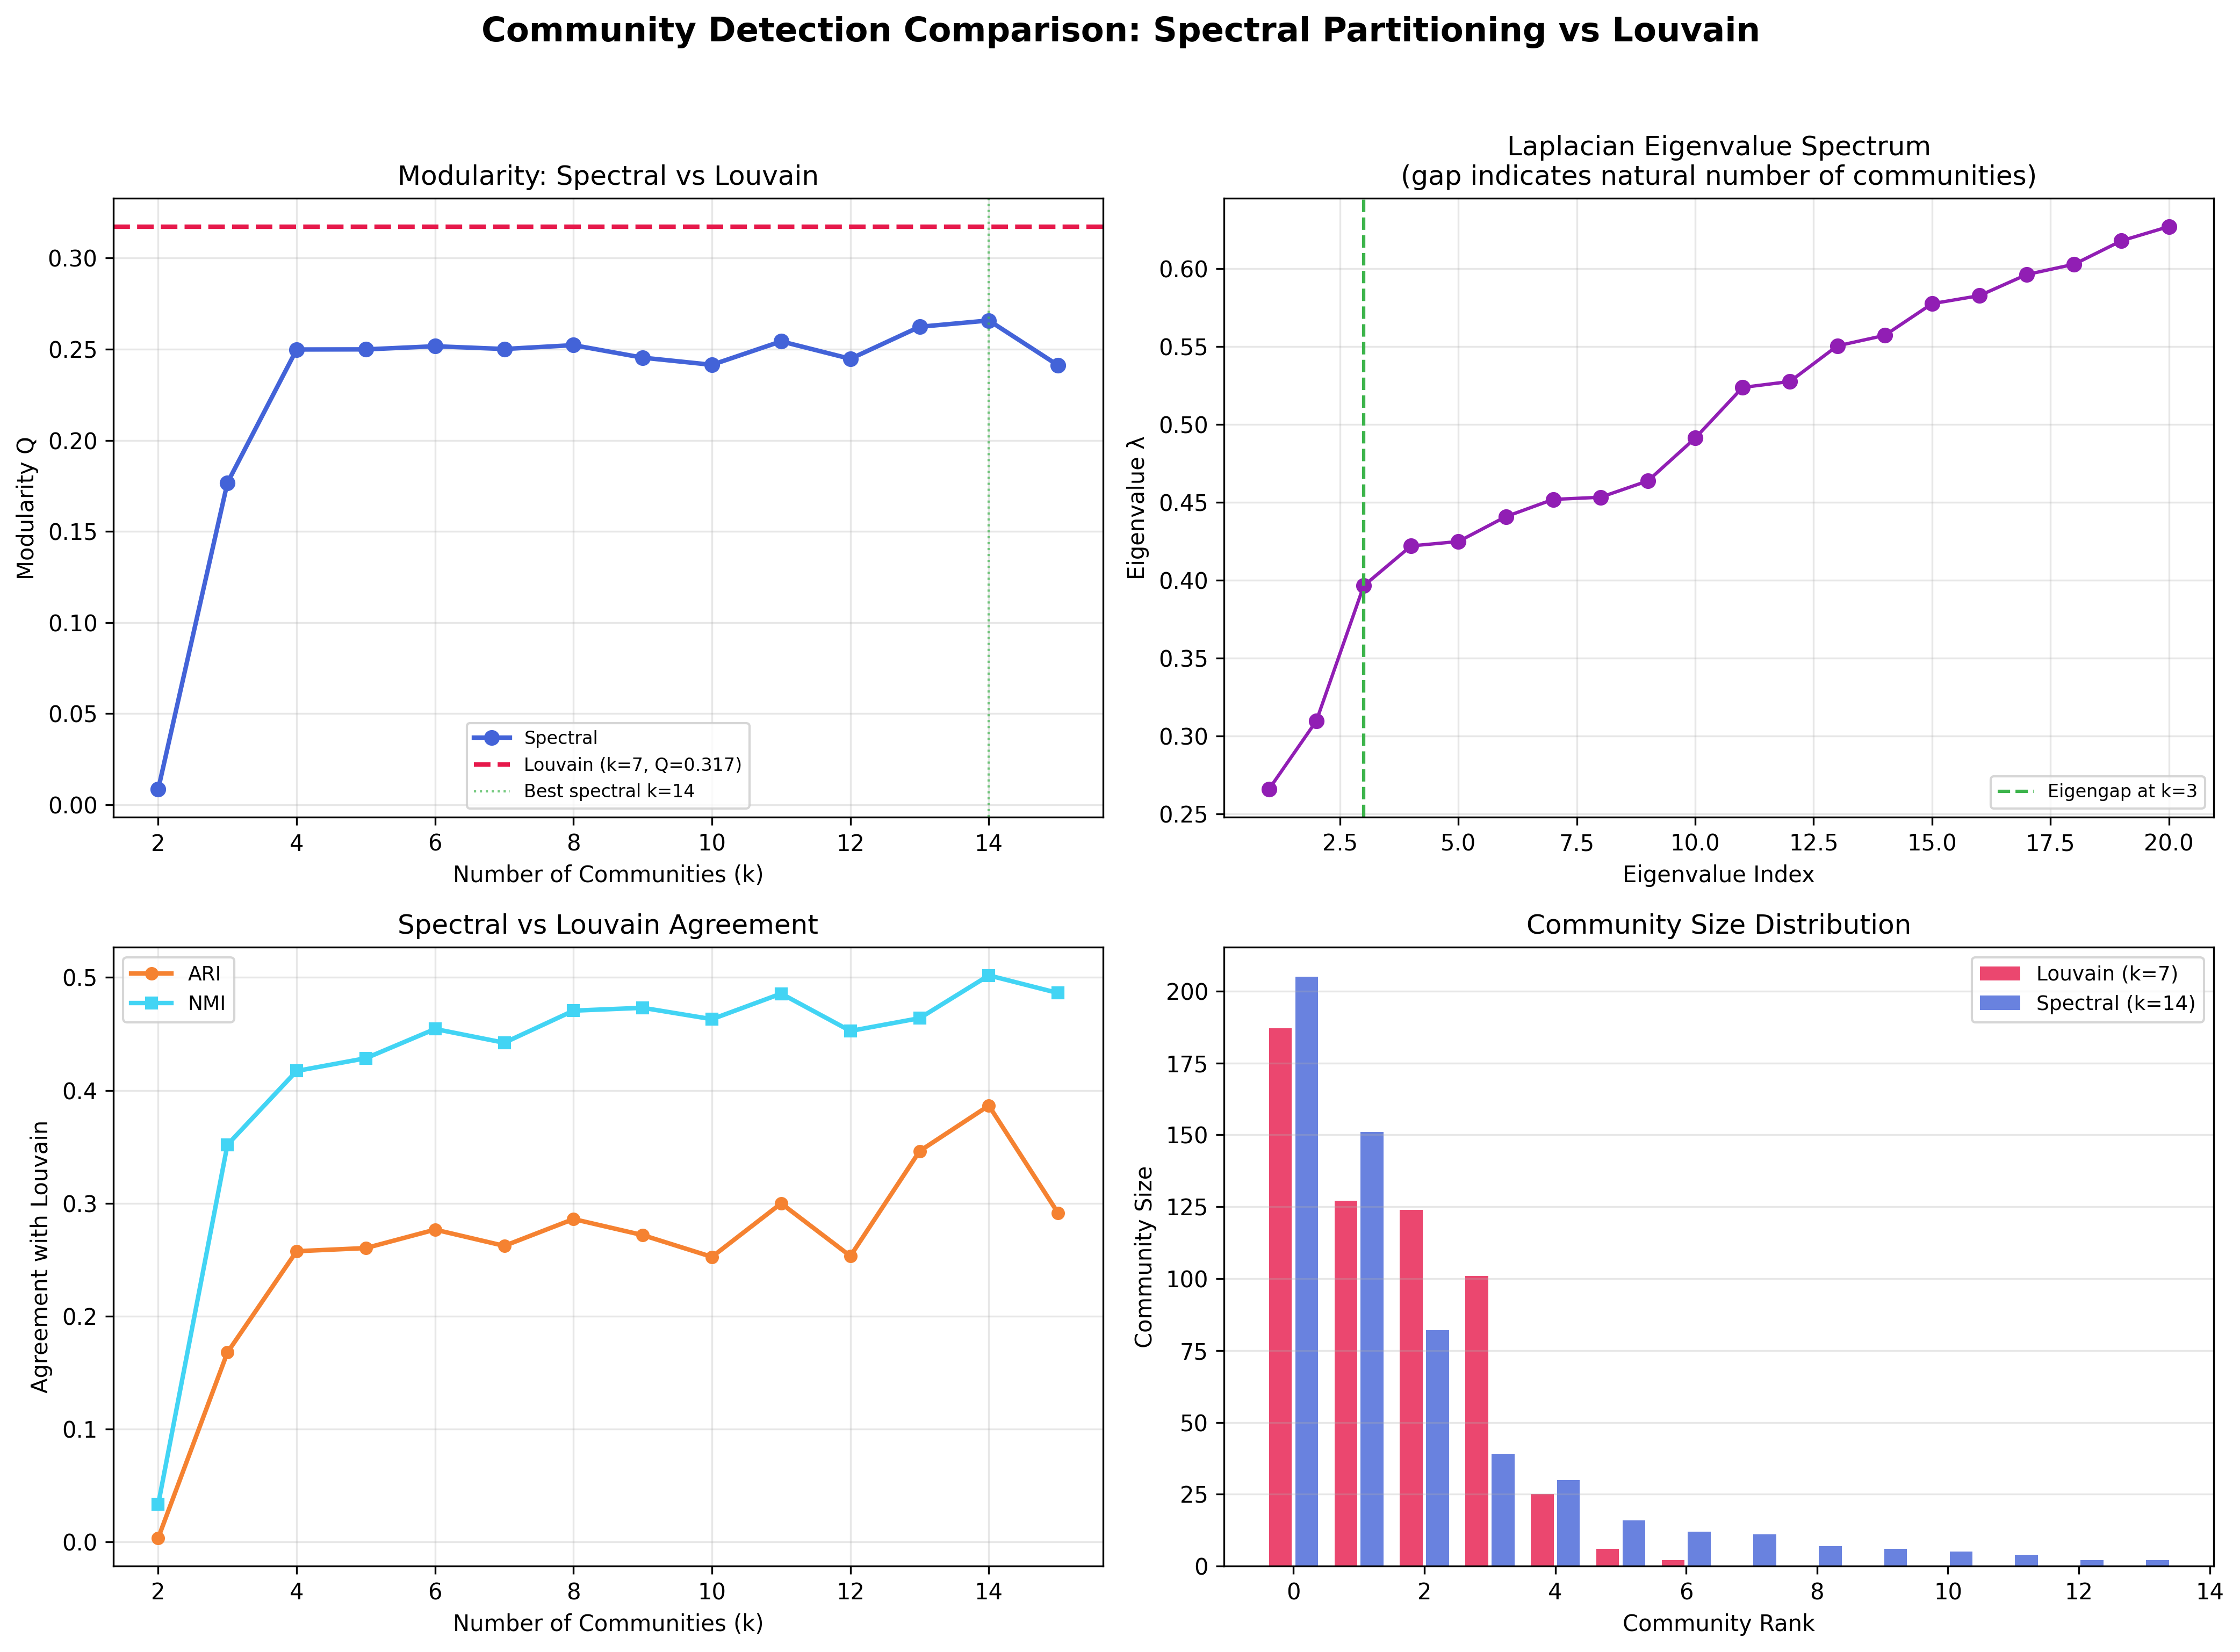
\includegraphics[width=\columnwidth]{figures/fig_spectral_vs_louvain.png}
\caption{Community detection comparison: spectral graph partitioning (Lecture~04) vs.\ Louvain. Top-left: Louvain achieves higher modularity at every $k$. Top-right: Laplacian eigenvalue spectrum with eigengap at $k=3$. Bottom-left: ARI/NMI agreement between methods. Bottom-right: community size distributions.}
\label{fig:spectral}
\end{figure}

\begin{figure}[!htbp]
\centering
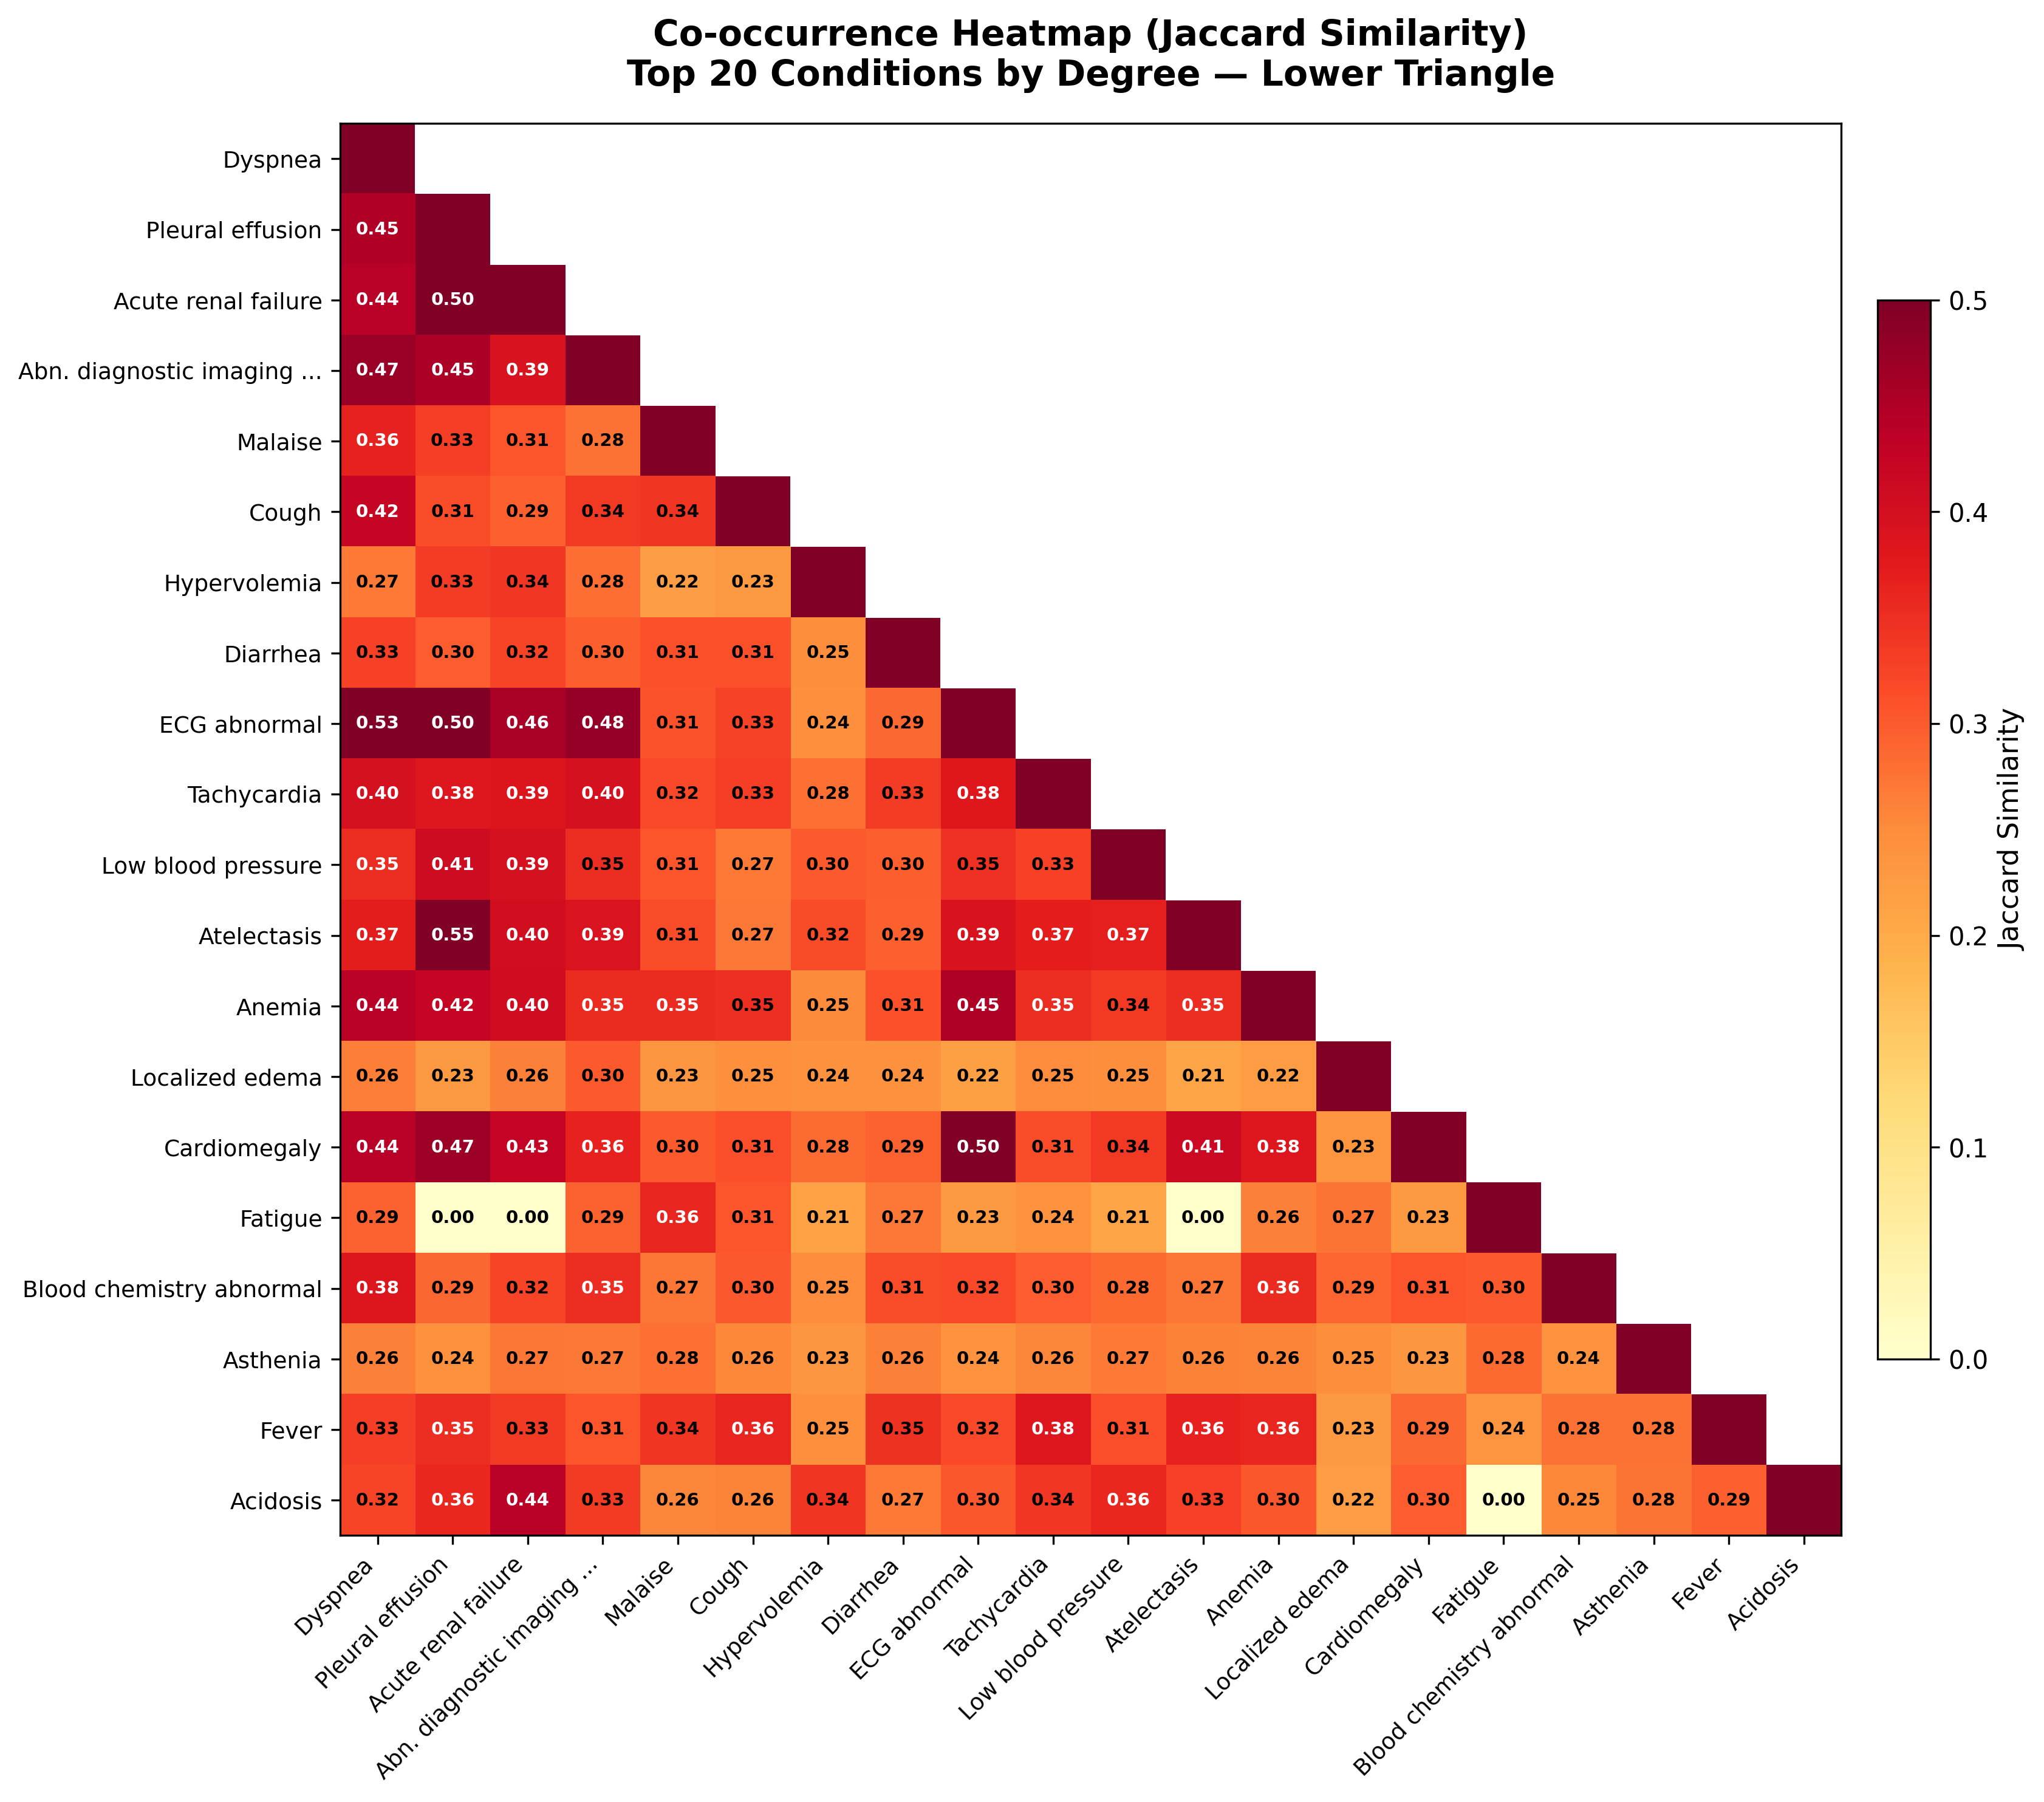
\includegraphics[width=\columnwidth]{figures/fig8_jaccard_heatmap.png}
\caption{Jaccard similarity heatmap (lower triangle) for the top 20 conditions by degree. Darker cells indicate stronger co-occurrence; values are annotated in each cell.}
\label{fig:heatmap}
\end{figure}


% ======================================================================
% SECTION 6: INTERPRETATIONS AND CONCLUSIONS
% ======================================================================
\section{Interpretations and Conclusions}

\subsection{Comorbidity Communities Reflect Clinical Disease Domains}

The Louvain algorithm identified 12 communities with modularity 0.317, indicating meaningful community structure (Figure~\ref{fig:network}, Table~\ref{tab:communities}, Figure~\ref{fig:communities}).
The four major communities are clinically coherent.
Community~4 (Cardiometabolic core, Figure~\ref{fig:zoomin}) groups essential hypertension, hyperlipidemia, T2D, and ECG abnormalities---precisely the metabolic syndrome cluster that clinicians recognize as the foundation of T2D complication risk.
Community~10 (Acute/Critical care) groups pleural effusion, acute renal failure, atelectasis, and tachycardia, representing the acute decompensation events that bring T2D patients to the hospital.
Community~2 (Renal) tightly groups end-stage renal disease, dialysis-related conditions, and CKD-specific anemia, reflecting the distinct clinical pathway of advanced nephropathy.

This structure confirms that comorbidity co-occurrence is not random but organized around recognizable disease domains (Figure~\ref{fig:heatmap}), consistent with Barab\'asi et al.'s network medicine framework~\cite{barabasi2011}.

\subsection{Spectral vs.\ Louvain Community Detection}

We compared spectral graph partitioning (Lecture~04) with Louvain across $k = 2$--$15$ (Figure~\ref{fig:spectral}).
The Laplacian eigenvalue spectrum shows a gap at $k = 3$, suggesting three coarse communities, but modularity peaks at $k = 14$ for spectral ($Q = 0.266$), still below Louvain's $Q = 0.317$ at $k = 7$ (automatically detected).
The moderate ARI ($0.39$) and NMI ($0.50$) between methods indicate partial agreement: both capture the cardiometabolic and renal clusters, but spectral partitioning tends to produce one or two oversized communities ($>$200 nodes) while fragmenting others into small groups ($<$10 nodes).
Louvain produces more balanced and clinically interpretable communities because its greedy modularity optimization naturally handles weighted edges and avoids the size imbalance inherent in spectral bisection.
We therefore use Louvain as our primary community detection method while noting that both approaches confirm the existence of distinct comorbidity clusters.

\subsection{Bridge Diagnoses as Complication Gateways}

The 52 bridge diagnoses (Table~\ref{tab:bridges}, Figure~\ref{fig:bridges}) identify conditions that connect separate disease communities.
Dyspnea, the top bridge (betweenness = 0.086, participation coefficient = 0.757), connects 5 communities because it can signal cardiac failure (Community~4), pulmonary complications (Community~10), anemia (Community~1), or general deconditioning (Community~3).
This makes dyspnea a clinically important warning sign---a patient presenting with new dyspnea may be transitioning from one disease domain to another.

Similarly, anemia (betweenness = 0.032, PC = 0.748) bridges the hematologic, renal, and cardiometabolic clusters, consistent with its role as both a cause and consequence of CKD, heart failure, and chronic disease.
These bridge diagnoses represent candidate conditions for targeted comorbidity screening in T2D patients.

\subsection{Temporal Gateways: The Metabolic Triad}

Essential hypertension dominates the temporal network with an outgoing strength of 52,193, meaning it precedes the largest number of downstream conditions across the most patients (Table~\ref{tab:gateways}, Figure~\ref{fig:temporal}).
Hyperlipidemia (42,370) and T2D itself (46,281) form the remaining members of what we term the ``metabolic triad''---the three conditions that temporally precede virtually all other T2D complications.
This is consistent with Jensen et al.'s population-level finding that metabolic conditions act as trajectory entry points~\cite{jensen2014}.

\subsection{Demographic Disparities}

The subgroup comparison (Table~\ref{tab:subgroups}, Figures~\ref{fig:subgroup_nets} and~\ref{fig:demographics}) reveals three patterns:

\begin{itemize}
    \item \textbf{Sex:} Female patients have denser networks (0.684 vs.\ 0.652) and more communities (9 vs.\ 7), suggesting a more fragmented comorbidity landscape with more distinct disease domains.
    \item \textbf{Age:} The 75+ group has the fewest communities (3), indicating that comorbidity clusters merge as patients age---older patients accumulate conditions across domains, eroding the boundaries between clusters.
    \item \textbf{Young patients:} The Under-60 group has the lowest density (0.640), reflecting fewer co-occurring conditions in younger T2D patients.
\end{itemize}

These structural differences suggest that comorbidity screening strategies may need to be age- and sex-specific.

\subsection{Network Topology}

The network exhibits small-world properties (Table~\ref{tab:global}): high clustering (transitivity = 0.427) with short average path length (2.197).
The diameter of 5 means that any two conditions in the network are at most 5 steps apart.
The degree distribution (Figure~\ref{fig:degree}) is right-skewed with a few high-degree hubs (dyspnea: degree 254, pleural effusion: 236) and many low-degree conditions, consistent with scale-free-like behavior observed in other disease networks~\cite{hidalgo2009}.

\subsection{Limitations}

\begin{itemize}
    \item \textbf{Single institution:} EHRShot data comes from Stanford Medicine, which may not generalize to other populations or healthcare systems.
    \item \textbf{Coding bias:} Conditions are recorded as billing codes, which may over-represent conditions with reimbursement incentives and under-represent conditions that are clinically noted but not coded.
    \item \textbf{Temporal granularity:} Condition dates reflect when codes were entered, not necessarily when symptoms began. Same-day co-diagnoses may reflect coding practices rather than true simultaneity.
    \item \textbf{Lifetime co-occurrence:} Our co-occurrence window captures chronic comorbidity but cannot distinguish conditions that co-occur due to shared pathophysiology from those that co-occur due to shared demographics (e.g., age-related conditions).
\end{itemize}

\subsection{Future Directions}

This structural analysis provides the foundation for predictive modeling using Graph Neural Networks in Project~2, where we will use the network structure to predict future comorbidity links.
Several extensions could strengthen the analysis:

\begin{itemize}
    \item \textbf{Link prediction:} Using the community structure and node embeddings (spectral or GNN-based) to predict which conditions a T2D patient is likely to develop next, enabling proactive screening.
    \item \textbf{Multilayer networks:} Incorporating medication and procedure data as additional node types would create a richer network capturing treatment patterns alongside disease co-occurrence, revealing drug--disease and procedure--disease associations.
    \item \textbf{Temporal dynamics:} Constructing time-windowed networks (e.g., yearly snapshots) would capture how comorbidity structure evolves as patients age, rather than collapsing all records into a single static network.
    \item \textbf{Multi-institutional validation:} Replicating this analysis on other OMOP-formatted EHR datasets (e.g., MIMIC-IV, UK Biobank) would test whether the community structure and bridge diagnoses generalize beyond Stanford Medicine.
\end{itemize}

\subsection{Conclusion}

We constructed and analyzed a weighted comorbidity network of 578 conditions among 1,354 T2D patients from the EHRShot dataset, applying a comprehensive suite of social network analysis techniques to uncover the hidden structure of disease co-occurrence.

Our analysis yielded four key findings.
First, community detection using the Louvain algorithm revealed 12 clinically coherent disease clusters (modularity $Q = 0.317$), with the cardiometabolic core (hypertension, hyperlipidemia, T2D, ECG abnormalities) forming the most densely connected community.
We validated this result against spectral graph partitioning from the course lectures, confirming that Louvain produces more balanced and interpretable communities for weighted networks.

Second, bridge diagnosis analysis identified 52 conditions---led by dyspnea (betweenness $= 0.086$, participation coefficient $= 0.757$), ECG abnormalities, and pleural effusion---that connect separate disease domains.
These bridges may serve as clinical ``canaries in the coal mine'': when a T2D patient develops one of these conditions, clinicians should screen for complications across multiple organ systems rather than treating the condition in isolation.

Third, temporal gateway analysis confirmed the ``metabolic triad'' (hypertension, T2D, hyperlipidemia) as the primary entry point to the complication landscape, with essential hypertension alone preceding over 52,000 patient-condition transitions.
This temporal ordering aligns with clinical guidelines that prioritize early blood pressure control in T2D management.

Fourth, demographic stratification revealed that female patients have more fragmented comorbidity landscapes (9 communities vs.\ 7 for males), while elderly patients ($75+$) show merging of disease clusters into just 3 broad communities---suggesting that comorbidity screening protocols should be tailored to patient demographics rather than applied uniformly.

From a methodological perspective, this project demonstrates that social network analysis techniques---originally developed for studying social relationships---transfer effectively to biomedical domains.
Concepts like community structure, bridge nodes, and centrality take on direct clinical meaning when applied to disease co-occurrence data.
The combination of Jaccard-weighted edges, Fisher's exact test filtering, and Louvain community detection provides a reproducible pipeline for mining comorbidity structure from any OMOP-formatted EHR dataset.

From a clinical standpoint, these results have practical implications for T2D management.
The identification of bridge diagnoses provides an evidence-based prioritization for comorbidity screening: when a T2D patient presents with dyspnea, anemia, or chest pain, the network structure suggests that clinicians should evaluate for complications across cardiac, pulmonary, renal, and hematologic domains simultaneously.
Similarly, the temporal gateway findings reinforce the importance of aggressive early management of hypertension and hyperlipidemia---not just for their own sake, but because they serve as the entry points through which the majority of downstream complications are reached.
The demographic differences in network structure further suggest that a one-size-fits-all approach to comorbidity screening may miss important patterns: younger patients may benefit from targeted monitoring of specific clusters, while older patients require broader multi-system surveillance as disease boundaries blur with age.

Looking ahead, the network structure and node-level metrics computed here will serve as input features for Graph Neural Network models in Project~2, where we aim to predict future comorbidity links and identify patients at risk of developing specific complications based on their current disease profile.
By combining the structural insights from this project with the predictive power of graph-based deep learning, we hope to develop tools that can alert clinicians to emerging comorbidity risks before they manifest as acute events.


% ======================================================================
% REFERENCES
% ======================================================================
\balance
\begin{thebibliography}{9}

\bibitem{hidalgo2009}
C.~A. Hidalgo, N.~Blumm, A.-L. Barab\'asi, and N.~A. Christakis,
``A dynamic network approach for the study of human phenotypes,''
\textit{PLoS Computational Biology}, vol.~5, no.~4, p.~e1000353, 2009.
\\\texttt{DOI: \href{https://doi.org/10.1371/journal.pcbi.1000353}{10.1371/journal.pcbi.1000353}}

\bibitem{jensen2014}
A.~B. Jensen, P.~L. Moseley, T.~I. Oprea, S.~G. Elles\o{e}, R.~Eriksson, H.~Schmock, P.~B. Jensen, L.~J. Jensen, and S.~Brunak,
``Temporal disease trajectories condensed from population-wide registry data covering 6.2 million patients,''
\textit{Nature Communications}, vol.~5, p.~4022, 2014.
\\\texttt{DOI: \href{https://doi.org/10.1038/ncomms5022}{10.1038/ncomms5022}}

\bibitem{barabasi2011}
A.-L. Barab\'asi, N.~Gulbahce, and J.~Loscalzo,
``Network medicine: a network-based approach to human disease,''
\textit{Nature Reviews Genetics}, vol.~12, no.~1, pp.~56--68, 2011.
\\\texttt{DOI: \href{https://doi.org/10.1038/nrg2918}{10.1038/nrg2918}}

\bibitem{blondel2008}
V.~D. Blondel, J.-L. Guillaume, R.~Lambiotte, and E.~Lefebvre,
``Fast unfolding of communities in large networks,''
\textit{Journal of Statistical Mechanics: Theory and Experiment}, vol.~2008, no.~10, p.~P10008, 2008.
\\\texttt{DOI: \href{https://doi.org/10.1088/1742-5468/2008/10/P10008}{10.1088/1742-5468/2008/10/P10008}}

\bibitem{guimera2005}
R.~Guimer\`a and L.~A.~N. Amaral,
``Functional cartography of metabolic networks,''
\textit{Nature}, vol.~433, no.~7028, pp.~895--900, 2005.
\\\texttt{DOI: \href{https://doi.org/10.1038/nature03288}{10.1038/nature03288}}

\bibitem{wornow2023}
M.~Wornow, R.~Thapa, E.~Steinberg, J.~Fries, and N.~Shah,
``EHRSHOT: An EHR benchmark for few-shot evaluation of foundation models,''
in \textit{Advances in Neural Information Processing Systems (NeurIPS)}, 2023.
\\\texttt{DOI: \href{https://doi.org/10.48550/arXiv.2307.02028}{10.48550/arXiv.2307.02028}}

\end{thebibliography}

\end{document}
